% -*- TeX -*- -*- ENG -*- -*- UNIX -*-

%#### My Input Data #######################################

% Choose the document class here:
% It has to be one of
%   DocumentClassBaMa    (Bachelor's or Master's thesis)
%   DocumentClassSeminar (seminar reports)

\documentclass[a4paper, % DIN A4 Format
	12pt, %Schriftgr��e
	twoside, %zweiseitiges Layout (linke und rechte Seiten)
	openright, %Kapitel fangen immer auf rechter Seite an
	cleardoublepage=empty, %evtl. eingef�gte Seiten sind leer (ohne Seitenzahl), alternativ: cleardoublepage=plain (mit Seitenzahl)
	numbers=noenddot, %hinter Kapitel- und Abschnittsnummern grunds�tzlich kein Punkt am Ende
	appendixprefix, %im Anhang bei Kapiteln eine Prefixzeile verwenden, z.B. "Anhang A"
	BCOR1.5cm, %Binderand
	bibliography=totoc %Literaturverzeichnis ins Inhaltsverzeichnis aufnehmen
	%idxtotoc %Indexverzeichnis ins Inhaltsverzeichnis aufnehmen
	]{scrbook} % Dokumentklasse aus KOMA-Paket, alternativ: scrartcl oder scrreprt

%############################################################### % Dokumentklasse bestimmen

\def\ausarbeitungsTypBachelor{Bachelor}
\def\ausarbeitungsTypMaster{Master}
\def\ausarbeitungsTypDiplom{Diplom}
\def\ausarbeitungsTypSeminar{Seminar}
\def\ausarbeitungsTypProSeminar{Pro-Seminar}

\def\bachelorArbeit{Bachelor's Thesis}
\def\masterArbeit{Master's Thesis}
\def\diplomArbeit{Diploma Thesis}
\def\seminarArbeit{Seminar Thesis}

\def\gradBachelor{Bachelor of Science}
\def\gradMaster{Master of Science}
\def\gradDiplom{Diplom-Informatiker} % Konstanten laden, z.B.: Begriffe wie Bachelor-Arbeit, Bachelor of Science, etc.

\usepackage[american]{babel}
%\usepackage[ansinew]{inputenc} %F�r deutsche Kodierung von Buchstaben �,�,�,� unter Windows (f�r Unix: 'latin1' statt 'ansinew') ansonsten muss man Folgendes schreiben:
% \"a f�r �, \"o f�r �, \"u f�r �, \ss f�r �.
%\usepackage{german} % unter anderem f�r bessere Silbentrennung

%#### My Input Data #######################################

% the following values have to be adapted for each thesis


% The following instruction defines the type of thesis or report, the following arguments are allowed:
% \ausarbeitungsTypBachelor		Bachelor's thesis
%\ausarbeitungsTypMaster			Master's thesis
% \ausarbeitungsTypDiplom			Diploma thesis
% \ausarbeitungsTypSeminar		Seminar report (Master's program)
% \ausarbeitungsTypProSeminar	Pro-Seminar report (Bachelor's program)
\def\ausarbeitungsTyp{\ausarbeitungsTypMaster}

\def\meinErstellungsdatum{August 2015} % day of completion, e.g. May 2009
\def\meinTitel{Modelling of long-term and conditional volatility dynamics in high-frequency returns at fixed trading time points us-ing a general Semi-GARCH model} % your title
\def\meinName{Xiaojing Hou} % your name
\def\meineStrasseHausNr{Hoehen Str.28} % street and house number
\def\meinePLZundOrt{33098 Paderborn} % zip code and city
\def\meinErstgutachter{Prof. Yuanhua Feng} % first supervisor, applies to seminars, too
\def\meinZweitgutachter{xxx} % second supervisor, irrelevant for seminars
\def\meinePDFStichwoerter{Template, technical articles, thesis, seminar} % key words

\def\titelDesSeminars{Software Engineering for Software-Intensive Systems} % seminar topic, apllies to seminars only

%############################################################### % Parameter wie Autor, Titel, Datum, Gutachter, etc.
\include{graphix}
\usepackage{ifthen} % Paket f�r if-then-else-Konstrukte

\usepackage{verbatim}  % z.B. f�r comment-Umgebung
\usepackage{natbib}    % f�r BibTeX mit dinat style (DIN 1505, Teil 2 und 3)   20.06.2015 shuo wang aktiviert
%\bibliographystyle{abbrvnat} %new style
%\bibliographystyle{dinat} %new style
%\bibliographystyle{abbrvnat} %new style
\bibliographystyle{apalike}
%\usepackage{bibgerm}   % f�r BibTeX mit deutschem style z.B. geralpha
%\usepackage{makeidx}   % f�r Index-/Stichwortverzeichnis
%\makeindex             % l�sst LaTeX die Indexeintr�ge sammeln
%\usepackage{epsfig}   % zum Einf�gen von EPS-Grafiken
\usepackage{array}     % weitere Hilfsmittel f�r Tabellen
\usepackage{multirow}    % table shuo wang added
\usepackage{booktabs}    % table shuo wang added
%\usepackage{graphicx} % ya suo biaoge
%\usepackage{float}    % f�r weitere Gleitumgebungen au�er table und figure
\renewcommand{\baselinestretch}{1.5} 
\usepackage{setspace}  % f�r 1-fachen, 1,5-fachen oder 2-fachen Zeilenabstand
%\floatstyle{plain}
%\floatname{sourcecode}{Code-Fragment}
%\newfloat{sourcecode}{htbp}{loc}[chapter] % neue Gleitumgebung f�r Quellcode


%Mathe
\usepackage{amsmath}
\usepackage{amsfonts}

\usepackage{bbm}
\newcommand{\IN}{\mathbbm{N}}           % nat�rliche Zahlen
\newcommand{\IZ}{\mathbbm{Z}}           % ganze      Zahlen
\newcommand{\IQ}{\mathbbm{Q}}           % rationale  Zahlen
\newcommand{\IR}{\mathbbm{R}}           % reelle     Zahlen
\newcommand{\IC}{\mathbbm{C}}           % komplexe   Zahlen
\newcommand{\IP}{\mathbbm{P}}           % Primzahlen

\renewcommand{\epsilon}{\varepsilon}                    % sch�neres Epsilon

\newcommand{\set}[1]{\left\{ #1 \right\}}               % Menge
\newcommand{\powerset}[1]{\wp\!\left(#1\right)}         % Potenzmenge
\newcommand{\abs}[1]{\left\lvert #1 \right\rvert}       % Betrag
\newcommand{\norm}[1]{\left\lVert #1 \right\rVert}      % Norm
\newcommand{\floor}[1]{\left\lfloor #1 \right\rfloor}   % floor
\newcommand{\ceil}[1]{\left\lceil #1 \right\rceil}      % ceiling

\newcommand{\signatur}[3]{#1:#2\,\rightarrow\,#3}     %Funktionen-Signatur


%Umgebungen
\newenvironment{bew}{\vspace{6pt}{\raggedright\textbf{Beweis: }}} {\newline\vspace{6pt}\hfill{$\square$}\vspace{6pt}\newline}

\usepackage{theorem}
%\theoremstyle{change} %vertauscht Nummer und Titel, z.B. statt "Def. 1.1" steht "1.1 Def."
\newtheorem{definition}{Definition}[chapter]
\newtheorem{satz}[definition]{Satz}
\newtheorem{korollar}[definition]{Korollar}
\newtheorem{lemma}[definition]{Lemma}
\newtheorem{theorem}[definition]{Theorem}
\newtheorem{bsp}[definition]{Beispiel}
{\theoremstyle{changebreak}\newtheorem{bspe}[definition]{Beispiele}} %mit neuer Zeile anfangen
 % einige mathematische Hilfskonstrukte und Vereinfachungen

%Formatierung
\newcommand{\clearemptydoublepage}{\newpage{\pagestyle{empty}\cleardoublepage}}
\usepackage{fancyhdr}
\pagestyle{fancy}
%\pagestyle{plain} %'headings' f�r Seitenzahl oben, Fu�zeile leer, 'plain' oder 'empty' auch m�glich
%\addtolength{\headwidth}{\marginparsep}
%\addtolength{\headwidth}{\marginparwidth}
%\addtolength{\headwidth}{3cm}
\renewcommand{\chaptermark}[1]{\markboth{\sc\thechapter. #1}{}}
\renewcommand{\sectionmark}[1]{\markright{\sl\thesection~#1}}
\lhead[\fancyplain{}{\leftmark}]{}
\rhead[]{\fancyplain{}{\rightmark}}
\lfoot[\fancyplain{\bf\thepage}{\bf\thepage}]{}
\rfoot[]{\fancyplain{\bf\thepage}{\bf\thepage}}
\cfoot[]{}

\fancypagestyle{plain}{% Neudefinition der plain-Seiten
\fancyhf{}
\fancyfoot[LE,RO]{\textbf{\thepage}}
\renewcommand{\headrulewidth}{0pt}
\renewcommand{\footrulewidth}{0pt}
}
 % Layout der Seiten, z.B. Kopf- und Fu�zeilendefinition


% ueberpruefen, ob wir pdflatex ausfuehren (geht nur bei Koma-Klassen)
\ifpdfoutput
{ 
% PDF wird genutzt
	
	\usepackage[pdftex]{graphicx,color}
	% eigene Farben f�r Links:
  %\definecolor{myLinkColor}{rgb}{0,0,.5}
  %\definecolor{myCiteColor}{rgb}{0,.5,0}
  %\definecolor{myFileColor}{rgb}{.5,0,0}
  %\definecolor{myURLColor}{rgb}{0,0,1}
  % Setzen aller Link-Farben auf Schwarz
  \definecolor{myLinkColor}{rgb}{0,0,0}
  \definecolor{myCiteColor}{rgb}{0,.5,0}
  \definecolor{myFileColor}{rgb}{0,0,0}
  \definecolor{myURLColor}{rgb}{0,0,0}
  \usepackage[pdftex,%
  						pdftitle={\meinTitel},%
  						pdfauthor={\meinName},%
  						pdfkeywords={\meinePDFStichwoerter},% Stichw�rter
  						plainpages=false,%
  						pdfpagelabels,% Seitenzahl als z.B. 'ii (4 of 40)' anstatt '4 of 40' darstellen
  						colorlinks=true,%
  						linkcolor=myLinkColor,%
  						citecolor=myCiteColor,%
  						filecolor=myFileColor,%
  						urlcolor=myURLColor,%
  						bookmarks,% Lesezeichen erstellen
  						bookmarksnumbered, % Lesezeichen nummeriert wie im Inhaltsverzeichnis
  						breaklinks, % Zeilenumbr�che bei Links erlauben
  						%pdfpagelayout={TwoColumnRight}% zweiseitiges fortlaufendes Layout
  						]{hyperref}
  \pdfcompresslevel=9 %Kompressionslevel fuer Text und Grafiken
  \DeclareGraphicsExtensions{.pdf, .png, .jpg, .tif, .mps} % Dateiendungen f�r Grafikdateien, geordnet nach Priorit�t f�r automatische Auswahl der richtigen Datei, falls Endung nicht angegeben
}
{
% Kein PDF
  
  \usepackage{graphicx}
  \usepackage{color}
  \usepackage[hypertex, bookmarks,% Lesezeichen erstellen
  						bookmarksnumbered, % Lesezeichen nummeriert wie im Inhaltsverzeichnis
  						breaklinks, % Zeilenumbr�che bei Links erlauben
  						]{hyperref}
  \DeclareGraphicsExtensions{.eps,.ps} % Dateiendungen f�r Grafikdateien
}

%--- hyphenation -----------------------------------------------------------------------------

% Silbentrennung f�r W�rter, in denen kein Bindestrich vorkommt
%--- hyphenation -----------------------------------------------------------------------------

% hyphenation for words without hyphens in them, i.e. not for words like stand-alone, hard-wired, etc.
\hyphenation{%
soft-ware
en-gi-nee-ring
} 

%----------------------------------------------------------------------------------------------

%----------------------------------------------------------------------------------------------
%shuo wang set paragraph
\setlength{\parskip}{10pt}
\setlength\parindent{0pt}


\begin{document}

% Verzeichnisse umbenennen von "...verzeichnis"; muss hier stehen, da sonst der Name nicht ge�ndert wird
%\renewcommand{\contentsname}{Inhalt}
%\renewcommand{\bibname}{Literatur}

\pagenumbering{roman} % r�mische Seitenzahlen, bevor der eigentliche Inhalt beginnt


%--- bastard title -------------------------------------------------------------------------------

\ifthenelse{
	\equal{\ausarbeitungsTyp}{\ausarbeitungsTypMaster}
	\OR
	\equal{\ausarbeitungsTyp}{\ausarbeitungsTypDiplom}
	}
	{
		%then: create a bastard title
		\thispagestyle{empty}
		\begin{center}
		{\vspace*{170pt}\Large\textbf{\meinTitel}}\\[30pt]
		by\\[15pt]
		{\large \meinName}
		\end{center}
		\clearpage
	}
	{
	 	%else: do nothing
	}


%--- Title page -------------------------------------------------------------------------------

\thispagestyle{empty}
\begin{titlepage}
\begin{center}
	
	\begin{minipage}{13.5cm}		
		
\includegraphics[height=3cm]{Images/TitlePage/uni-logo}\\
		\textsf{
   		 \hspace*{2.0cm} Fakult\"at f\"ur Betriebswirtschaftslehre \\
		\hspace*{2.0cm} Fachgebiet �konometrie und quantitative Methoden \\
		\hspace*{2.0cm} Warburger Stra\ss e 100 \\
     	\hspace*{2.0cm} 33098 Paderborn
		}
	\end{minipage}\\[60pt]
  
  
  \begin{doublespace}
		{\Huge\textbf{\meinTitel}}\\[30pt]
	\end{doublespace} 
  
    
  \ifthenelse{\equal{\ausarbeitungsTyp}{\ausarbeitungsTypMaster}}
	{
		%then:
		{\Large \masterArbeit }\\[6pt]
		%--Submitted to the Software Engineering Research Group\\
		%--in Partial Fulfillment of the Requirements for the\\
		%--Degree of\\[6pt]
  	    
  	   % {\Large \gradMaster}\\[30pt]
  	
	}
	{
	 	%else:
	 	\ifthenelse{\equal{\ausarbeitungsTyp}{\ausarbeitungsTypDiplom}}
		{
			%then:
			{\Large \diplomArbeit }\\[6pt]
	  	Submitted to the Software Engineering Research Group\\
		  in Partial Fulfillment of the Requirements for the\\
		  Degree of\\[6pt]
	  	{\Large \gradDiplom}\\[30pt]
		}
		{
		 	%else:
		 	\ifthenelse{\equal{\ausarbeitungsTyp}{\ausarbeitungsTypBachelor}}
			{
				%then:
				{\Large \bachelorArbeit }\\[6pt]
		  	Submitted to the Software Engineering Research Group\\
		    in Partial Fulfillment of the Requirements for the\\
		    Degree of\\[6pt]
		  	{\Large \gradBachelor}\\[30pt]
			}
			{
			 	%else:
			 	\ifthenelse{\equal{\ausarbeitungsTyp}{\ausarbeitungsTypSeminar}
			 							\OR
			 							\equal{\ausarbeitungsTyp}{\ausarbeitungsTypProSeminar}
			 						 }
				{
					%then:
					{\Large \seminarArbeit }\\[6pt]
			  	Submitted to the Software Engineering Research Group\\
			  	in Partial Fulfillment of the Requirements for the\\
			  	\ifthenelse{\equal{\ausarbeitungsTyp}{\ausarbeitungsTypSeminar}}
			  	{
			  		Seminar\\[6pt]
			  	}
			  	{
			  		%else
			  		Pro-Seminar\\[6pt]
			  	}
			  	{\Large \titelDesSeminars}\\[10pt]
				}
				{
				 	%else: sollte nie der Falls sein
				 	{\Large Kind of thesis unknown }\\[42pt]
				}
			}
		}
	}  
  
  
  by\\
  {\scshape\large \meinName}\\
  \meineStrasseHausNr\\\meinePLZundOrt\\[20pt]
  
  Thesis Supervisor:\\
  
\ifthenelse{\equal{\ausarbeitungsTyp}{\ausarbeitungsTypSeminar}\OR{\equal{\ausarbeitungsTyp}{\ausarbeitungsTypProSeminar}}}
{
	%then: nur Erstgutachter
	{\large \meinErstgutachter}\\[20pt]
}
{
 	%else: Erst- und Zweitgutachter
 	{\large \meinErstgutachter}\\
  and\\
  {\large \meinZweitgutachter}\\[10pt]
}
  
  %{\today} % heutiges Datum \meinErstellungsdatum
  {Paderborn, {\today}}
\end{center}
\end{titlepage}
\clearpage


%---Erkl�rung----------------------------------------------------------------------------------

\ifthenelse{
	\equal{\ausarbeitungsTyp}{\ausarbeitungsTypMaster}
	\OR
	\equal{\ausarbeitungsTyp}{\ausarbeitungsTypDiplom}
	\OR
	\equal{\ausarbeitungsTyp}{\ausarbeitungsTypBachelor}
	}
{
	%then: Erkl�rung einf�gen
	
	%\clearemptydoublepage

	\chapter*{Declaration}\vspace{-24pt}
	
	(Translation from German)\newline
	
	\noindent I hereby declare that I prepared this thesis entirely on my own and have not used outside sources
	without declaration in the text. Any concepts or quotations applicable to these sources are
	clearly attributed to them. This thesis has not been submitted in the same or substantially similar
	version, not even in part, to any other authority for grading and has not been published elsewhere.

	\section*{Original Declaration Text in German:}

	\section*{Erkl\"arung}
	
	Ich versichere, dass ich die Arbeit ohne fremde Hilfe und ohne Benutzung anderer als der
	angegebenen Quellen angefertigt habe und dass die Arbeit in gleicher oder \"ahnlicher Form
	noch keiner anderen Pr\"ufungsbeh\"orde vorgelegen hat und von dieser als Teil einer
	Pr\"ufungsleistung angenommen worden ist. Alle Ausf\"uhrungen, die w\"ortlich oder sinngem\"a\ss~
	\"ubernommen worden sind, sind als solche ge\-kenn\-zeich\-net.\\[27pt]
	
	
	\begin{center}
		\begin{tabular}{l p{0.1\textwidth} r}
		  \cline{1-1} \cline{3-3}
		  \begin{minipage}[t]{0.4\textwidth}
		    \centering
		    City, Date
			\end{minipage}
			&
			\begin{minipage}[t]{0.2\textwidth}
			\end{minipage}
			&
			\begin{minipage}[t]{0.4\textwidth}
			  \centering
			  Signature
			\end{minipage}
		\end{tabular}
	\end{center}
}
{
	%else: nichts tun
}


%---Inhaltsverzeichnis-------------------------------------------------------------------------
%\clearemptydoublepage
\tableofcontents

% Please change only this file to adapt your document's structure.

%--- list of figures ----------------------------------------------------------------------

\ifthenelse{
	\equal{\ausarbeitungsTyp}{\ausarbeitungsTypMaster}
	\OR
	\equal{\ausarbeitungsTyp}{\ausarbeitungsTypDiplom}
	\OR
	\equal{\ausarbeitungsTyp}{\ausarbeitungsTypBachelor}
	}
{
	%then: add a list of figures
	
	%\clearemptydoublepage
	\listoffigures
}
{
	%else: do nothing
}


%--- list of tables ------------------------------------------------------------------------

\ifthenelse{
	\equal{\ausarbeitungsTyp}{\ausarbeitungsTypMaster}
	\OR
	\equal{\ausarbeitungsTyp}{\ausarbeitungsTypDiplom}
	\OR
	\equal{\ausarbeitungsTyp}{\ausarbeitungsTypBachelor}
	}
{
	%then: add a list of tables
	
	%\clearemptydoublepage
	\listoftables
}
{
	%else: do nothing
}

%\setcounter{secnumdepth}{4} % create section numbers up to level 4, e.g.: 3.2.5.4, usually not necessary


%######################## Chapter 1 ######################################################
\cleardoublepage
\pagenumbering{arabic} % use arabic page numbers again

\chapter{Introduction}\label{secIntroduction}
Trading off risks against returns appears to be essential and vital for making a financial decision. Hence the econometric analysis of risk (volatility) becomes an important part in forecasting market tendency and supporting making financial decisions, such as portfolio diversification, risk management and derivative pricing. In the last 20 years volatility was a research hotspot in financial industry. Volatility is regarded as a parameter for evaluating the risk of assets return. Generally, the stronger the volatility is, the higher the risk is.

In the traditional financial models, the variance of the time series is always assumed as constant. However, it is found that the volatilities of financial time series have always the features of ``clustering'' and ``fat tails'' \citep{Mandelbrot1963,EugeneF.Fama1965}. These features obviously are not consistent with the assumption of constant, so the traditional econometric methods cannot analyze the financial time series efficiently in practice. To overcome this problem, several economists have carried out studies on researching and developing frameworks for evaluating volatility. Since Engle introduced the autoregressive conditional heteroskedasticity (ARCH) model \citep{Engle1982}, the extensions of ARCH model appeared and spread rapidly. Among the carried out researches, the Generalized ARCH (GARCH) model and its derivatives are most widely used \citep{Bollerslev1986}.

 According to many studies \citep{Gourieroux1992,Eubank1993}, in parametric model, the preselected model might be too restricted or too low-dimensional, which may not fit unexpected features and cause the misspecification. However, in nonparametric model, the parameters of the model cannot be estimated, and the model cannot be explained due to lack of specific functions. Instead of parametric model or nonparametric model, recently proposed semi-parametric model will be introduced in details in this paper, which introduces a smooth scale function into the standard GARCH model. This model does not need a prespecified function and is less sensitive to model misspecification. At the same time, the model can be also explained \citep{Di2011}.

In this paper, the definition, estimation, some properties of semi-parametric model and the methods of bandwidth selection are discussed. Furthermore, based on the study of the semi-parametric GARCH model and semi-parametric asymmetric power ARCH model, which are introduced by Feng \citep{Feng2004,FengYuanhua;Sun2013}, the semi-parametric exponential GARCH and component GARCH models are originally defined. Then, the discussed semi-parametric models, i.e. Semi-APARCH, Semi-EGARCH and Semi-CGARCH models, are applied to the returns of BMW and Allianz from January 2006 to September 2014. Different from other papers, to get the more exact analyzing results the fixed trading time points are used in this paper.

The scope of this paper is as follows. In section 2, the parametric models are introduced. The semi-parametric models are described in section 3. Section 4 reports the application of the semi-parametric models to the returns of BMW and Allianz and the empirical results on the volatility of the selected data sets. Finally, this paper is concluded in section 5.

%######################## Chapter 2 ######################################################
%\clearemptydoublepage
%\chapter{Fundamentals}

carpe diem carpe diem carpe diem carpe diem carpe diem carpe diem carpe diem carpe diem 
carpe diem carpe diem carpe diem carpe diem carpe diem carpe diem carpe diem carpe diem 

\section{Layout}

carpe diem carpe diem carpe diem carpe diem carpe diem carpe diem carpe diem carpe diem 
carpe diem carpe diem carpe diem carpe diem carpe diem carpe diem carpe diem carpe diem 
carpe diem carpe diem carpe diem carpe diem carpe diem carpe diem carpe diem carpe diem 
carpe diem carpe diem carpe diem carpe diem carpe diem carpe diem carpe diem carpe diem 
carpe diem carpe diem carpe diem carpe diem carpe diem carpe diem carpe diem carpe diem 
carpe diem carpe diem carpe diem carpe diem carpe diem carpe diem carpe diem carpe diem 
carpe diem carpe diem carpe diem carpe diem carpe diem carpe diem carpe diem carpe diem 
carpe diem carpe diem carpe diem carpe diem carpe diem carpe diem carpe diem carpe diem 


carpe diem carpe diem carpe diem carpe diem carpe diem carpe diem carpe diem carpe diem 
carpe diem carpe diem carpe diem carpe diem carpe diem carpe diem carpe diem carpe diem 
carpe diem carpe diem carpe diem carpe diem carpe diem carpe diem carpe diem carpe diem 
carpe diem carpe diem carpe diem carpe diem carpe diem carpe diem carpe diem carpe diem 
carpe diem carpe diem carpe diem carpe diem carpe diem carpe diem carpe diem carpe diem 
carpe diem carpe diem carpe diem carpe diem carpe diem carpe diem carpe diem carpe diem 
carpe diem carpe diem carpe diem carpe diem carpe diem carpe diem carpe diem carpe diem 
carpe diem carpe diem carpe diem carpe diem carpe diem carpe diem carpe diem carpe diem 
carpe diem carpe diem carpe diem carpe diem carpe diem carpe diem\footnote{carpe noctem}

carpe diem carpe diem carpe diem carpe diem carpe diem carpe diem carpe diem carpe diem 
carpe diem carpe diem carpe diem carpe diem carpe diem carpe diem carpe diem carpe diem 
carpe diem carpe diem carpe diem carpe diem carpe diem carpe diem carpe diem carpe diem 
carpe diem carpe diem carpe diem carpe diem carpe diem carpe diem carpe diem carpe diem 
carpe diem carpe diem carpe diem carpe diem carpe diem carpe diem carpe diem carpe diem 
carpe diem carpe diem carpe diem carpe diem carpe diem carpe diem carpe diem carpe diem 
carpe diem carpe diem carpe diem carpe diem carpe diem carpe diem carpe diem carpe diem 


carpe diem carpe diem carpe diem carpe diem carpe diem carpe diem carpe diem carpe diem 
carpe diem carpe diem carpe diem carpe diem carpe diem carpe diem carpe diem carpe diem 
carpe diem carpe diem carpe diem carpe diem carpe diem carpe diem carpe diem carpe diem 
carpe diem carpe diem carpe diem carpe diem carpe diem carpe diem carpe diem carpe diem 
carpe diem carpe diem carpe diem carpe diem carpe diem carpe diem carpe diem carpe diem 
carpe diem carpe diem carpe diem carpe diem carpe diem carpe diem carpe diem carpe diem 
carpe diem carpe diem carpe diem carpe diem carpe diem carpe diem carpe diem carpe diem 
carpe diem carpe diem carpe diem carpe diem carpe diem carpe diem carpe diem carpe diem 
carpe diem carpe diem carpe diem carpe diem carpe diem carpe diem carpe diem carpe diem 
carpe diem carpe diem carpe diem carpe diem carpe diem carpe diem carpe diem carpe diem 
carpe diem carpe diem carpe diem carpe diem carpe diem carpe diem carpe diem carpe diem 
carpe diem carpe diem carpe diem carpe diem carpe diem carpe diem carpe diem carpe diem 
carpe diem carpe diem carpe diem carpe diem carpe diem carpe diem carpe diem carpe diem 
carpe diem carpe diem carpe diem carpe diem carpe diem carpe diem carpe diem carpe diem 
carpe diem carpe diem carpe diem carpe diem carpe diem carpe diem carpe diem carpe diem 
carpe diem carpe diem carpe diem carpe diem carpe diem carpe diem carpe diem carpe diem 
carpe diem carpe diem carpe diem carpe diem carpe diem carpe diem carpe diem carpe diem 
carpe diem carpe diem carpe diem carpe diem carpe diem carpe diem carpe diem carpe diem 
carpe diem carpe diem carpe diem carpe diem carpe diem carpe diem carpe diem carpe diem 
carpe diem carpe diem carpe diem carpe diem carpe diem carpe diem carpe diem carpe diem 
carpe diem carpe diem carpe diem carpe diem carpe diem carpe diem carpe diem carpe diem 


carpe diem carpe diem carpe diem carpe diem carpe diem carpe diem carpe diem carpe diem 
carpe diem carpe diem carpe diem carpe diem carpe diem carpe diem carpe diem carpe diem 
carpe diem carpe diem carpe diem carpe diem carpe diem carpe diem carpe diem carpe diem 
carpe diem carpe diem carpe diem carpe diem carpe diem carpe diem carpe diem carpe diem 
carpe diem carpe diem carpe diem carpe diem carpe diem carpe diem carpe diem carpe diem 
carpe diem carpe diem carpe diem carpe diem carpe diem carpe diem carpe diem carpe diem 
carpe diem carpe diem carpe diem carpe diem carpe diem carpe diem carpe diem carpe diem 
carpe diem carpe diem carpe diem carpe diem carpe diem carpe diem carpe diem carpe diem 
carpe diem carpe diem carpe diem carpe diem carpe diem carpe diem carpe diem carpe diem 
carpe diem carpe diem carpe diem carpe diem carpe diem carpe diem carpe diem carpe diem 
carpe diem carpe diem carpe diem carpe diem carpe diem carpe diem carpe diem carpe diem 
carpe diem carpe diem carpe diem carpe diem carpe diem carpe diem carpe diem carpe diem 
carpe diem carpe diem carpe diem carpe diem carpe diem carpe diem carpe diem carpe diem 


carpe diem carpe diem carpe diem carpe diem carpe diem carpe diem carpe diem carpe diem 
carpe diem carpe diem carpe diem carpe diem carpe diem carpe diem carpe diem carpe diem 
carpe diem carpe diem carpe diem carpe diem carpe diem carpe diem carpe diem carpe diem 
carpe diem carpe diem carpe diem carpe diem carpe diem carpe diem carpe diem carpe diem 
carpe diem carpe diem carpe diem carpe diem carpe diem carpe diem carpe diem carpe diem 
carpe diem carpe diem carpe diem carpe diem carpe diem carpe diem carpe diem carpe diem 
carpe diem carpe diem carpe diem carpe diem carpe diem carpe diem carpe diem carpe diem 
carpe diem carpe diem carpe diem carpe diem carpe diem carpe diem carpe diem carpe diem 
carpe diem carpe diem carpe diem carpe diem carpe diem carpe diem carpe diem carpe diem 
carpe diem carpe diem carpe diem carpe diem carpe diem carpe diem carpe diem carpe diem 
carpe diem carpe diem carpe diem carpe diem carpe diem carpe diem carpe diem carpe diem 
carpe diem carpe diem carpe diem carpe diem carpe diem carpe diem carpe diem carpe diem 
carpe diem carpe diem carpe diem carpe diem carpe diem carpe diem carpe diem carpe diem 
carpe diem carpe diem carpe diem carpe diem carpe diem carpe diem carpe diem carpe diem 


carpe diem carpe diem carpe diem carpe diem carpe diem carpe diem carpe diem carpe diem 
carpe diem carpe diem carpe diem carpe diem carpe diem carpe diem carpe diem carpe diem 
carpe diem carpe diem carpe diem carpe diem carpe diem carpe diem carpe diem carpe diem 
carpe diem carpe diem carpe diem carpe diem carpe diem carpe diem carpe diem carpe diem 
carpe diem carpe diem carpe diem carpe diem carpe diem carpe diem carpe diem carpe diem 
carpe diem carpe diem carpe diem carpe diem carpe diem carpe diem carpe diem carpe diem 
carpe diem carpe diem carpe diem carpe diem carpe diem carpe diem carpe diem carpe diem 
carpe diem carpe diem carpe diem carpe diem carpe diem carpe diem carpe diem carpe diem 
carpe diem carpe diem carpe diem carpe diem carpe diem carpe diem carpe diem carpe diem 
carpe diem carpe diem carpe diem carpe diem carpe diem carpe diem carpe diem carpe diem 
carpe diem carpe diem carpe diem carpe diem carpe diem carpe diem carpe diem carpe diem 
carpe diem carpe diem carpe diem carpe diem carpe diem carpe diem carpe diem carpe diem 
carpe diem carpe diem carpe diem carpe diem carpe diem carpe diem carpe diem carpe diem 


carpe diem carpe diem carpe diem carpe diem carpe diem carpe diem carpe diem carpe diem 
carpe diem carpe diem carpe diem carpe diem carpe diem carpe diem carpe diem carpe diem 
carpe diem carpe diem carpe diem carpe diem carpe diem carpe diem carpe diem carpe diem 
carpe diem carpe diem carpe diem carpe diem carpe diem carpe diem carpe diem carpe diem 
carpe diem carpe diem carpe diem carpe diem carpe diem carpe diem carpe diem carpe diem 
carpe diem carpe diem carpe diem carpe diem carpe diem carpe diem carpe diem carpe diem 
carpe diem carpe diem carpe diem carpe diem carpe diem carpe diem carpe diem carpe diem 
carpe diem carpe diem carpe diem carpe diem carpe diem carpe diem carpe diem carpe diem 

%######################## Chapter 2 ######################################################
%\clearemptydoublepage
\chapter{Parametric models}\label{secGarchmodel}
It is known that, volatility clustering exists in financial time series, and the distribution of random variables appears the fat tails. Mandelbrot observed the pattern of thick tails or fat tails of stock prices fluctuation, which was not consistent with the traditional assumption of normal distribution, by study the stock price index \cite{Mandelbrot1963}. 
Fama uggested that the financial market returns had the property of volatility clustering. It means that volatility is not only dynamic but also clustered, which appears strong in one certain period but weak in another period. The reasons for these phenomena could be traced back to speculation, political changes, government monetary and fiscal policy, and etc. \cite{EugeneF.Fama1965}. “Volatility clustering” and “fat tails” cannot be explained by the traditional economic models, which assume the variance is constant, until the Autoregressive Conditional Heteroscedasticity (ARCH) model was introduced by Engle (1982) \cite{Bollerslev1992}.


Different from the traditional models, ARCH model suggests that the conditional variance could change over time as a function of past errors with the unconditional variance remaining constant \cite{Engle1982}. ARCH model soon became an important tool of volatility measurement, because it improved the traditional model and fit reality better. However, there are some drawbacks in ARCH model. In practical applications of the ARCH model, a relatively long lag in the conditional variance equation is often required, which might lead to increase in complexity of estimating parameters and decrease the freedom degree. When the lag order is high, estimating a totally free lag distribution will often violate the constraint of non-negativity parameters. But the restrict condition is exactly needed in this model to ensure conditional variance to be non-negative \cite{Bollerslev1986}. Therefore, there are many economists tried to improve ARCH models. Among these researches, the generalized ARCH (GARCH) model, which is introduced by Bollerslev (1986), is the most widely well known one with a better framework to study time-varying volatility in financial markets. 

\section{Parametric GARCH model}
GARCH model added the lagged conditional variances to ARCH model, so that it has a longer memory and a more flexible lag structure than ARCH model.

\subsection{Definitions and basic properties}
In GARCH model, $F_{t-1}$ denote the set of the past information. The GARCH process is presented in \ref{equ2.1},

\begin{equation} 
\label{equ2.1}
	\varepsilon_t =  \eta_t h_t^{1/2}    \qquad    \varepsilon_{t}|F_{t-1}\sim N(0,h_{t})_,
 \end{equation} 
 
in which $\varepsilon_t$ is a random variables; $\eta_t$ are i.i.d. random  variables with zero mean and unit variance; $h_{t}$ means the conditional variance of $\varepsilon_{t}$ and is defined as follow:

\begin{equation} 
h_t = \omega + \sum_{i=0}^p \alpha_i \varepsilon_{t-1}^2 + \sum_{j=1}^q\beta_j h_{t-j},
\end{equation} 

where $\omega>0$ is the variances intercept parameter; $p>0$ is the order of ARCH parameters; $q \geq 0$ is the order of GARCH parameters; $\alpha$ and $\beta$ ( $ \alpha_i \geq 0, i=1, \dots ,p; \beta_j \geq 0, j=1,\dots,q$) are two vectors of unknown parameters respectively \cite{Bollerslev1986}.

From the model we can see that, GARCH model contains the lagged conditional variances in addition to ARCH model. When  $q=0$, the process is ARCH model; if $ p = q = 0$, this process is a simple white noise; while $\sum_{i=1}^p\alpha_i <1$, this process is an infinite dimensional ARCH  $(\infty)$. That means that ARCH is a special form of GARCH process. Most of the cases, a high order ARCH model can be replaced by a low order GARCH model without breaking the constraint of non-negativity by estimating too many parameters. For example, In the application of ARCH (p) model, sometimes the value of p is very high; but for GARCH (p, q) model, $p=1, q=1$ are enough to achieve the same outcome \cite{Engle1986}


In the paper from Engle, he introduced the stationary of GARCH model. As it is known, a process $\lbrace X_{t} \rbrace$  is weakly stationary,  if $i) E(X_{t}^{2}) < \infty$  for all  $t \in T$ ,$ ii) E(X_{t})$  and $cov(X_t,X_{t+s})$  are independent of $t$ for $s \in Z, t \in T$ \cite{Bougerol1992}.

So the GARCH $(p,q)$ process with $E\left( \varepsilon_t \right) =0, Var(\varepsilon_t) = \omega(1-  \sum_{i=1}^p\alpha_i - \sum_{j=1}^q\beta_j )^{-1}$ and $cov(Y_t,Y_s)=0$ for $t \neq s$ is wide-sense stationary if and only if $\sum_{i=1}^p\alpha_i + \sum_{j=1}^q\beta_j < 1 $ \cite{Bollerslev1986}

\subsection{Estimation of GARCH model}

Usually, the maximum likelihood estimation is most widely used to estimate GARCH model. Besides the condition of stationary, to estimate GARCH model, a very important assumption is finite fourth-order moment, which ensures the existence of the squared returns variance. Assuming GARCH model is a normal process:
 
\begin{equation}
E(\varepsilon_t^4)=\frac{3\omega^2(1+\alpha_1+\beta_1)}{(1-\alpha_1-\beta_1)(1-\beta_1^2-2\alpha_1\beta_1-3\alpha_1^2)}_.
\end{equation}

Under this condition, $E(\varepsilon_t^4)<\infty$ if and only if $3\alpha_1^2+2\alpha_1\beta_1+\beta_1^2<1$ for GARCH(1,1) mode \cite{Milhj2012}.  

Letting  $\theta=(\omega, \alpha_1, ..., \alpha_p,\beta_1,..., \beta_q)$, the conditional Gaussian log-likelihood function is defined as follows:

\begin{equation}
 L(\theta) = \frac{1}{n}\sum_{t-1}^nl_t,
\end{equation}

where

\begin{equation}
l_t =-\frac{1}{2}ln(h_t^2(F_{t-1};\theta))-\frac{\varepsilon_t^2}{2h_t^2(F_{t-1};\theta)}_.
\end{equation}

Then maximize $L(\theta)$ by calculating and putting the partial derivatives to zero. After n times iteration, the approximated value (MLE) of $\theta$ is obtained, which is denoted as $\hat{\theta}$.

The maximum likelihood method is used by most of cases in GARCH family. Based on the assumption of normal distribution, GARCH model can partially explain the clustering and fat tails properties of the returns’ unconditional distribution. However, after the standardized by GARCH model, the residuals also have the properties of clustering and fat tails, which is not consistent with the normal assumption. So Bollerslev and Nelson used student-t distribution and generalized error distribution (GED) instead of normal distribution to estimate GARCH models \cite{Bollerslev1986}\cite{Nelson1991}. When we estimate other GARCH models, which will be discussed below as examples, the main method is the same, maximum likelihood method. The most significant difference is the assumption of the distribution. 

Although a simple GARCH model can solve the problem of the ARCH model with high-order linear declining lag structure, it also has some obvious drawbacks.  The two constraint conditions of GARCH model, parametric non-negativity and bounded, restrict its applicability. The assumption of non-negative parameters raises the difficulty of estimation. Also with this assumption, the GARCH model cannot well explain the asymmetry of volatility and leverage effects. In order to extend the application of GARCH model, many GARCH derivatives appeared aiming at different problems. For example, to explain the asymmetry of volatility, the exponential GARCH model (EGARCH) was proposed by Nelson \cite{Nelson1991}, and threshold GARCH (TGARCH) was suggested by Zakorian \cite{Zakoian1994}. Ding, Granger and Engle introduced the APARCH model \citep{Ding1993}, which are able to explain the leverage effects in financial market better. Engle and Lee defined the component GARCH (CGARCH) model to exactly interpret the shock influences to the long-run and the short-run volatility respectively \cite{0-19-829683-5}.

\section{Parametric asymmetric power ARCH model}

Generally, if a data series follows the normal distribution, we can characterize it by its first two moments. However, if the error of the data follows a non-normal distribution, then higher moments of skewness, kurtosis have to be applied, which describes the data beyond to adequately. In this instance, other power transformations appeared to be more appropriate than squared term \cite{McKenzie1999}. Ding, Granger and Engle (1993) further studied the autocorrelation of square returns and absolute returns based on GARCH model and Taylor model. It is found that, long lags between absolute or square returns are more correlated than the returns themselves for the return process \cite{stephen1986modelling}. Furthermore, $|r_{t}|^{d}$ has the largest autocorrelation when d is around 1, but smaller monotonically one when d deviates from 1. Based on this they imposed an asymmetric GARCH model, asymmetric power ARCH model, which enables the power of the heteroskedasticity equation to be estimated from the data.


The parametric asymmetric power ARCH model is defined by

\begin{equation}
h_{t}^{\delta/2} = \omega + \sum_{i=1}^{p} \alpha_{i}(|\varepsilon_{t-i}|-\gamma_{i}\varepsilon_{t-i})^{\delta} + \sum_{j=1}^{q}\beta_{j}h_{t-j}^{\delta/2},
\end{equation}

where $\omega>0, \delta\geq0, \alpha_{i}\geq0, i=1, \ldots, p, -1<\gamma_{i}<1, i=1, \ldots, p, \beta_{j}\geq0.j=1, \ldots, q$. $\gamma$ is the leverage parameter, which takes the asymmetric news impact on the volatility into account,  and $\delta$ is the parameter for the power term, which is a suitable positive number.

This model exhibits a power transformation of the conditional standard deviation process, which can linearize nonlinear models. It also reveals the asymmetric absolute residuals, which can reflect the leverage effect of the stock market returns.


In APARCH model, when $\gamma_{t}$ is conditional normal, and 

\begin{equation}
\frac{1}{\sqrt{2\pi}}\sum_{i=1}^{p}\alpha_{i} \lbrace\left(1 + \gamma_{i} \right)^\delta + (1-\gamma)^{\delta}\rbrace2^{\frac{\delta-1}{2}}\Gamma (\frac{\delta+1}{2}) + \sum_{j=1}^{q}\beta_{j}<1,
\end{equation}

which is the condition to ensure the existence of $Eh_{t}^{\delta/2}$ and $E|\varepsilon_{t}|^{\delta}$, then when $\delta\geq2$, $\varepsilon_t$   is covariance stationary (sufficient condition) \cite{Ding1993}.


In the cases of the values of $\delta$ and $\gamma_{i}$ are changed, APARCH model derives into several models, the GJR-GARCH model, the TS-GARCH model(Taylor and Schwert model), the NGARCH model (Nonlinear GARCH model) and the TGARCH model (threshold GARCH model).

When $\delta=2,\gamma_{i}=0$, the APARCH model turns into a GARCH model with the covariance stationary for  $\varepsilon_{t}$ as $\sum_{i=1}^{p}\alpha_{i} + \sum_{j=1}^{q}\beta_{j}<1$ \cite{Bollerslev1986}.

When $\delta = 2, \gamma_{i}\neq 0$, the APARCH model can be named as the GJR (Glosten, Jagannathan and Runkle, 1993) model 

\begin{equation}
h_{t}=\omega + \sum_{i=1}^{p}\alpha_{i}\varepsilon_{t-i}^{2}+\gamma_{i}\varepsilon_{t-i}^{2}I(\varepsilon_{t-i}<0)+\sum_{j=1}^{q}\beta
_{j}h_{t-j},
\end{equation}

with the  covariance stationary for $\varepsilon_{t}$ as $\sum_{i=1}^{p}\alpha_{i}[1+\gamma_{i}^{2}]+\sum_{j=1}^{q}\beta_{j}<1$.

This model uses the indicator function I to simulate the asymmetric influence of the positive and negative shocks on the conditional variance \cite{Glosten1993}.

When $\delta=1,\gamma_{i}=0$, the APARCH model transforms into the TS-GARCH model

\begin{equation}
h_{t}^{1/2} = \omega + \sum_{i=1}^{p}\alpha_{i}|\varepsilon_{t-i}|+\sum_{j=1}^{q}\beta_{j}h_{t-j}^{1/2},
\end{equation}

with the covariance stationary for  $\varepsilon_{t}$, the same TS-GARCH model, as  $\sqrt{\frac{2}{\pi}} \sum_{i=1}^{p}\alpha_{i} + \sum_{j=1}^{\alpha}\beta_{j}<1$ \cite{Zakoian1994}

\section{Parametric exponential GARCH model}

It is considered that, GARCH model has taken the focus on the magnitude matters of excess return, but ignored the information of directions. Moreover, it is proven by empirical evidence that the direction does impact on volatility. Especially for broad-based equity indices and bond market indices, it is observed that market declines forecast higher volatility than comparable market increases do \cite{Engle2001}. In addition, the estimated coefficients often violate the parameter restrictions in GARCH model. It is also found that the left tail of the returns distribution was fatter than the right one. The reason is generally considered as the asymmetric response of investors to “good news” and “bad news” \cite{Jondeau2003}. To solve this problem Nelson (1991) imposed the exponential GARCH model.

Instead of making $h_{t}$  a linear combination of positive random variables, EGARCH model ensure that $h_{t}$  remains nonnegative by making $ln(h_{t})$ linear in some function g of time and lagged $\eta_{t}$‘s.

The exponential GARCH model can be written as follows:

\begin{equation}
ln(h_t) =\omega + \sum_{i=1}^p\alpha_ig(\eta_{t-i})+\sum_{j=1}^q\beta_jln(h_{t-j}),
\end{equation}

where

\begin{equation}
g(\eta_{t}) \equiv \theta\eta_t + \gamma[\mid\eta_t\mid-E\mid\eta_t\mid]. 
\end{equation}

In this model, $\beta\equiv 1 $; $\alpha$ and $\beta$ are real, non-stochastic and scalar sequences; $g(\eta_t)$ is a i.i.d. random sequences with zero mean \cite{Malmsten2004}.

EGARCH model provides a good solution for the problems of GARCH. There is no constraint for parameters. The function $g(\eta_t)$ contains two parts, $\gamma[|\eta_t|-E|\eta_t|]$ that define the size effect, and  $\theta\eta_t$   that defines the sign effect of the shocks on volatility. The size effect is a typical ARCH effect, but the sign effect is asymmetrical. For example, the leverage effect (Black, 1976), which means that volatility rises in response to negative shocks and falls in response to positive ones. 

According to the Theorem 2.1 from Nelson, when $\gamma$  and $\theta$  do not equal to zero at the same time, the EGARCH process is strictly stationary and ergodic if and only if $\sum_{i=1}^p\alpha_t^2 < \infty$. 

The estimation of EGARCH model is mostly same as the estimation of GARCH model. The difference between them is that, in EGARCH model, the generalized error distribution (GED) is used. Because this distribution includes the normal as special case; and when the process is strictly stationary and the distribution of  $\eta_t$ is not too fat tailed, $h_t$ and $\varepsilon_t$ have finite unconditional moments of arbitrary order \cite{Nelson1991}.

\section{Parametric component GARCH model}

It is known that the stock prices always fluctuate around an average value. This phenomenon is called mean-revert. It is also found that mean-revert of short-term volatility is more rapid than for the long-term one \cite{XinzhongXuandStephenJ.Taylor1994}. In order to explain this different response between short-term and long-term, Engle and Lee (1999) imposed component GARCH model. In this model, the conditional variance is decomposed into a permanent and transitory component. So that the model can be used to investigate the long-run and short-run movements of volatility affecting securities.

The component GARCH model is defined by

\begin{equation}
h_{t}=q_{t}+\sum_{i=1}^{p}\alpha_{i}(\varepsilon_{t-i}^{2}-q_{t-i}) + \sum_{j=1}^{q}\beta_{j}(h_{t-j}-q_{t-j}),
\end{equation}

\begin{equation}
q_{t} = \omega + \rho q_{t-1}  +\varphi(\varepsilon_{t-1}^{2}-h_{t-1})
\end{equation}

where $q_{t}$ the permanent component of the conditional variance and $(h_{t-j}-q_{t-j})$ is the transitory component of the conditional variance \citep{Ghalanos2011}. $(\alpha + \beta)$ is the mean-revert of $s_{t}$. In terms of economy, the smaller the mean-reverting rate, the less persistent the expected volatility to market shocks in the past. That means, when the market receives the information of shocks, volatility responses quickly but has lower persistence. If $0<(\alpha + \beta)<1$, the mean-reverts of short-run volatility component is zero at a geometric rate of  $(\alpha + \beta)$; If $0<\rho<1$,  the long-run volatility component follows an AR process, and will converge to a constant level defined by $\omega/(1-\rho)$.  In this model, the long-run component is more persistent than the short-run one, i.e., $0<(\alpha + \beta)<p<1$

In GARCH model, the conditional variance must be non-negative. This condition is also required in component GARCH model. But this is not demanded by $s_{t}$, which can be positive or negative over time to exhibit the self-correction feature of the mean-reverting volatility process. The condition of stationary in GARCH model is  $\sum_{i=1}^{p}\alpha_{i} + \sum_{j=1}^{\alpha}\beta_{j}<1$ , besides which this stationary condition also includes $(\alpha + \beta)(1-\rho)+\rho<1$ and requires $\rho<1,(\alpha + \beta)<1$ in component model. When $\rho=1$, the mean series is not a covariance stationary process, but also is still a strictly stationary and ergodic process.

From the above analysis, the stationary conditions of component GARCH model can be concluded as $0<(\alpha + \beta)< \rho<1, 0<\varphi<\beta,\alpha>0,\beta>0,\alpha_{0}>0,\varphi>0$,  But they are just sufficient conditions, not necessary ones \cite{0-19-829683-5}.
   




%######################## Chapter 3 ######################################################
%\clearemptydoublepage
\chapter{Semi-parametric volatility models}\label{semiparaGarch}

The GARCH model has many advantages. The function form is accessible, and parameters could be easily estimated. If the model assumptions were correct, the estimation is consistent with reality. However, the drawbacks of parametric models are more disgusting. Firstly, a preselected parametric model may not fit unexpected features, due to too restricted or too low dimensional. Secondly, sometimes the regression function seems to be too complicate or difficult to be defined. Thirdly, because different sequence will be witnessed when different conditional distribution is selected in the process of prediction by using parametric models, there will most possibly exist the problem of misspecification, which may result in a excessively high model bias and loss of efficiency, unless the assumed function perfectly matches the true error distribution \citep{Di2011}.

Gourieroux and Monfort had firstly inserted the conditional mean and conditional variance into a nonparametric model, in which the function form is not given.  This model can improve the defects of parametric models. Correspondingly, it is less sensitive to model misspecification and can offer a flexible tool in analyzing unknown regression relationships 
\citep{Gourieroux1992}. In nonparametric regression models, both the error distribution and the functional form of the mean function are not pre-specified. It will be more useful when the regression function seems to be very complex or a suitable function form cannot be found \citep{Eubank1993}. However, the nonparametric models lose some functions, which can be realized by parametric models. Due to lack of specific function forms, the parameters of the model cannot be estimated. Furthermore, the model cannot be explained. Excess variable estimates could rise up because of poor consideration of nonparametric models, especially for small sample size. So a new model, semi-parametric model, is proposed.

Semi-parametric model consists of not only the nonparametric part but also parametric part. Semi-parametric GARCH model selects the nonparametric form for the scale function and the parametric part for conditional variance lags. Then it does not need a pre-specified function form and is less sensitive to model misspecification. At the same time, the parametric part can also explain the models \citep{Di2011}.

\section{Semi-GARCH model}

\subsection{Definition of Semi-GARCH model}

Semi-GARCH model combines a smooth scale function with the standard GARCH model:

\begin{equation}
\label{eq:3.1}
Y_{t} = \mu + \sigma(x_{t})\varepsilon_{t},
\end{equation}

where $\mu$ is an unknown constant; $x_{t}=t/n; \sigma(x)>0$ is the nonparametric component, a smooth, bounded scale function; and $\lbrace\varepsilon_{t}\rbrace$ is the parametric component. The conditional variance of $\lbrace\varepsilon_{t}\rbrace$ is assumed to follow a GARCH(p, q) process:

\begin{equation}
\label{equ3.3}
h_{t}=\omega + \sum_{i=1}^{p}\alpha_{i}\varepsilon_{t-i}^{2} + \sum_{j=1}^{q}\beta_{j}h_{t-j},
\end{equation}

where $h_t^{1/2}$ is the conditional standard deviations of the standardized process $\varepsilon_t$; $ \omega>0;  \alpha_{1}, \ldots ,\alpha_{p}\geq0$ and $\beta_{1},\ldots,\beta_{q}\geq0$.    To estimate the scale function, $E(\varepsilon_{t}^{8})<\infty$ is assumed to ensure \ref{equ3.3} strictly stationary, which implies in particular that $\sum_{i=1}^p\alpha_i+\sum_{j=1}^q\beta_j<1$ \citep{Feng2004}.

The semi-parametric model provides us a tool to decompose financial risk into an unconditional component $\sigma(x_t)$ , a conditional component $h_{t}^{1/2}$  and the i.i.d. innovations $\eta_{t}$.

\subsection{Estimation of Semi-GARCH model}
\label{subsec3.1.2}
The estimation of Semi-GARCH model can combine the nonparametric estimation of the Y's local variance  $v(x)=\sigma^{2}(x)$,with parametric estimation of the unknown parameter vectors $\theta = (\alpha_{0},\alpha_{1},\ldots,\alpha_{p},\beta_{1},\ldots,\beta_{q})$.

At first, the scale function can be estimated by some nonparametric regression approaches without any parametric assumptions. In this model the kernel estimation will be used. If the constant mean $\mu$ is replaced by a sooth function g, we can get a nonparametric regression with scale change and dependence

\begin{equation}
\label{equ3.5}
Y_t= g(x_t)+\sigma(x_t)\varepsilon_t,
\end{equation}

where ${\varepsilon_t}$ is a zero mean stationary process.


Therefore, Equation \ref{eq:3.1} can be transformed into a general nonparametric regression problem at first. Letting $ r_{t}=Y_{t}-\mu$, $X_{t}=r_{t}^{2}$ and $\xi_{t}=\varepsilon_{t}^{2}-1 \geq -1$, which are zero mean stationary time series errors. Then the model \ref{eq:3.1} can be rewritten as 

\begin{equation}
\label{equ3.4}
 X_{t} = v(x_{t} )+ v(x_{t})\xi_{t}.
\end{equation}


Letting $\hat{\mu }=\bar{y}$ and $\hat{x}_{t} = \hat{r}_{t}^{2}$, in which $\hat{r_{t}}$ is then defined by $\hat{r}_{t}=y_{t}-\bar{y}$. A Nadaraya-Watson kernel regression, which has been proposed by Nadaraya (1964) and Watson (1964), is defined by

\begin{equation}
\hat{v}(x)=\frac{\sum_{t=1}^{n}K(\frac{x_t-x}{b})\hat{r}_t}{\sum_{t=1}^{n}K(\frac{x_t-x}{b})}=:\sum_{t=1}^nW_t\hat{r}_t,
\end{equation}

where $W_t$ is the weighting function  $W_t= \frac{K(\frac{x_t-x}{b})}{\sum_{t=1}^{n}K(\frac{x_t-x}{b})} $; $K(u)$ is a second order kernel function with compact support [-1,1]; and b is the bandwidth, the size of the weights \citep{Fan1993}. 

According to the above assumptions, the estimator $\varepsilon_{t}$  is now replaced by the standardized residuals

\begin{equation}
\hat{\varepsilon_t }=\hat{r_t}/\hat{\sigma }(x_t)=(y_t-\bar{y})/\hat{\sigma}(x_t). 
\end{equation}

Then the estimator of parametric vector $\theta$ can be obtained by the standard maximum likelihood method, which has been introduced in section 2. A suitable model can also be selected by using other methods, e.g. the akaike information criterion (AIC), the bayesian information criterion (BIC) and etc. \citep{Feng2004}.



\subsection{ Asymptotic properties of $\hat{v}$}
To calculate the asympototic optimal bandwidth, several assumptions must be made:
 \begin{enumerate}
    \item $E(\varepsilon_{t}^{8})<\infty$ ensures the process strictly stationary, and $\eta \sim N(0,1)$\citep{Ling2002}.
    \item The second derivative of $v(x)$ exists and is continuous on $[0,1]$.
    \item The kernel $K(u)$ is a continuous function, which is symmetric around zero and defined in $[-1, 1]$.
    
    \item When the sample volume $n \rightarrow \infty $, the bandwidth $b \rightarrow 0 $ and $nb \rightarrow \infty $. Then both of the bias B and the variance V approaches zero.
  
\end{enumerate}
Define $R(K)= \int K^{2}(u)du$ and $I(K)=\int u^{2}K(u)du$ . Under these assumptions, the asymptotic bias and the asymptotic variance can be obtained.
The asymptotic bias B of $\hat{v}(x)$ is:

\begin{equation}
\label{equ3.6}
B=E[\hat{v}(x)-v(x)] = \frac{I(K)v''(x)}{2}b^{2}+o(b^{2}).
\end{equation}
The asymptotic variance V of $\hat{v}(t)$ can be expressed as:

\begin{equation}
\label{equ3.7}
V=var[\hat{v}(x)]=R(K)\frac{v(x)}{nb}+o(\frac{1}{nb}).
\end{equation}   

From equation \ref{equ3.6} and \ref{equ3.7} we can see that, the bias $B(x)=O(b^2)$ and the variance $V(x)=O(nb)^{-1}$. The bias has the positive correlation with the bandwidth, whereas the variance has the negative correlation with the bandwidth. The higher the $v(x)$, the larger the variance; and the more complex the $v(x)$, the larger the bias.
Then the asymptotic MISE can be calculated by:
\begin{equation}
MISE = \int(B^{2}+V)dt=\frac{I^{2}(K)R(V''(x))}{4}b^{4} + \frac{R(K)}{nb} + o[max(b^{4},\frac{1}{nb})].
\end{equation}
By minimizing the dominant part of the asymptotic MISE, the asymptotically optimal bandwidth of $\hat{v}$  is
\begin{equation}
b=(\frac{R(K)}{I^{2}(K)R(V''(x))})^{1/5}n^{-1/5}.
\end{equation}
When the bandwidth $b=n^{-1/5}$, we can get $\hat{v}(x)=v(x)[1+O_{p}(n^{-2/5})]$  and $MISE=O(n^{-4/5})$ \citep{Gasser1984,Fan1991}.

\subsection{The selection of the bandwidth}
Applying the estimator $\hat{v}$  requires the specification of kernels and bandwidth. Optimal kernels have been obtained analytically. The selection of bandwidth becomes the most important problem when applying nonparametric regression estimators such as kernel estimators. The regression works well, only if the bandwidth is suitable. Because the kernel estimation uses the points around $x_{0}$  to estimate the scale function, a kernel regression is usually biased. The larger the bandwidth, the larger the square bias because further points from $x_{0}$ are used, but the smaller the variance because more observations are used for estimation. The bandwidth should be optimized to balance the variance and bias. The optimal bandwidth is the one, which can minimize the mean squared error (MSE) or mean integrated squared error (MISE) \citep{Gasser1991}. 

There are many methods available to optimize bandwidth, e.g. Cross-Validation (CV), Generalized CV (GCV), plug-in and etc. In this paper, CV and plug-in will be introduced in detail.

\paragraph{Cross-Validation (CV)}

The Cross-Validation method is also called “leave-one-out”.  This method estimates the MSE by leaving one observation out at each time point. The main idea of CV is that, the estimation of $v(x_{t})$ is without using $(x_{t},\hat{r_{t}})$, rather assess the quality of the estimation with other observations. 

Define the estimation errors by $\lambda_{-t}=(x_{t},b)=\hat{r}_{t}-\hat{v}^{-t}(x_{t})$. The function to calculate CV is:
\begin{equation}
CV(b) = \sum_{t=1+t_{0}}^{n-t_{0}}\lambda_{-t}^{2}(x_{t},b)=\sum_{t=1+t_{0}}^{n-t_{0}}[\hat{r}_{t}-\hat{v}^{-t}(x_{t})]^{2},
\end{equation}
where $\hat{v}^{-t}(x_t)=\sum_{j=1,j\neq t}^{n}\frac{K(\frac{x_{j}-x_{t}}{b})\hat{r}_{j}}{\sum_{j=1,j \neq t}^{n}K(\frac{x_{j}-x_{t}}{b})}$ is the “leave-one-out’’ estimator of $v(x_{t})$.

Letting $0<h_{min}<h_{max}<1, \bigtriangleup h=(h_{max}-h_{min})/m$, where m is an integer. Then the optimal bandwidth can be obtained by calculating the value of CV at $h=h_{min}, h=h_{min} + \bigtriangleup h, h=h_{min} + 2\bigtriangleup h, \ldots, h=h_{max}$. The optimal bandwidth is the one, at which CV(b) is minimized \citep{Sarda1993}.

Cross-Validation is the most simple method for bandwidth selection and easy to understand. However, this method has large variability, which leads often a suboptimal non-parametric fit of the regression function. For example, the selected bandwidth by CV is often very large. Sometimes the resulted band width can be very small and wrong \citep{Altman1995}. 

\paragraph{Plug-in bandwidth selected method}

In this method, some adapted assumptions are required.


\begin{enumerate}
    \item The function $v(x)$ is strictly positive on [0,1] and exist at least continuous fourth moment.    
    \item $v''$ is estimated with a symmetric fourth order kernel for estimating the second derivative with compacted sup-port [-1,1].
    \item The bandwidth b satisfied $b \rightarrow 0$  and $nb^{5} \rightarrow \infty $  as $n \rightarrow \infty$.
\end{enumerate}

Denote $c_{f}=f(0)$, where $f(\tau)=(2\pi)^{-1}\sum_{k=-\infty}^{\infty}exp(ik\tau)\gamma_{\varepsilon}(k)$ is the spectral density of $\varepsilon_{t}$  with $\gamma_{\varepsilon}(k)$ is the autocovariance function of $\varepsilon_{t}$ . Then the asymptotic optimal bandwidth can be rewritten as 

\begin{equation}
b_{A} =(2\pi c_{f} \frac{R(K)}{I^{2}(K)}\frac{I(v^{2})}{I((v'')^2)})^{1/5}n^{-1/5} = Cn^{-1/5},
\end{equation}

where

\begin{equation}
c_{f}=\frac{E(\varepsilon_{t}^{4})}{3\pi}\frac{(1-\sum_{j=1}^{q}\beta_{j})^{2}}{(1-\sum_{i=1}^{p}\alpha_{i}-\sum_{j=1}^{q}\beta_{j})^{2}}
\end{equation}
 
with the assumption, the functions $\phi(z)=1-\sum_{i=1}^{max(p,q)}\alpha_{i}z^{i}$ and $\varphi(z)=1-\sum_{j=1}^{max(p,q)}\beta_{j}z^{j}$ have no common roots. $\hat{E}(\varepsilon_t^{4})=\sum_{t=1}^{n}\hat{\varepsilon}_{t}^{4}/n$ is a nonparametric estimator of $\varepsilon_{t}^{4}$ \citep{Feng2004}.

This method starts from the asymptotic optimal bandwidth $b_{0}= Cn^{-1/5}$ with C=0.5, then follows iteration process. In the j-th iteration: step 1, calculating $\hat{v}$  and $\hat{\theta}$  with the bandwidth $b_{j-1}$; step 2, calculating $\hat{E}(\varepsilon^{4})$ and $\hat{I}(v)^{2}$  with   $\hat{I}(v)^{2} = \frac{1}{n}\sum_{t=n_{1}}^{n_{2}}\hat{v}(x_{t})^{2}$, where $n_{1}$  and $n_{2}$ denote the integer part of [na] and [n(1-a)] respecyively, in which [a, 1-a] is the compacted support of the mean integrated squared error (MISE). In this calculation, the selected bandwidth is $b_{\varepsilon,j}=b_{v,j}=b_{j-1}^{5/4}$; step 3, calculating $\hat{c}_{f}$  from $\hat{\theta}$  and $\hat{E}(\varepsilon^{4})$; step 4, calculating $\hat{I}((v'')^{2})$, where $\hat{v}''$  is a kernel estimator of   $v''$  with $\hat{I}((v'')^{2})= \frac{1}{n}\sum_{t=n_{1}}^{n_{2}}\hat{v}''(x_{t})^{2}$, in which $\hat{v}''$ is obtained by using the bandwidth $b_{d,j}=b_{j-1}^{5/7}$; step 5, improve $b_{j-1}$  by 
\[ b_{A} =(2\pi \hat{c}_{f} \frac{R(K)}{I^{2}(K)}\frac{\hat{I}(v^{2})}{\hat{I}((v'')^2)})^{\frac{1}{5}}n^{-\frac{1}{5}}; \]

step 6, setting $j=j+1$ and repeating the iteration until  a) convergence is reached, where the condition $|b_{j} - b_{j-1}| <1/n$  is used as a criterion for the convergence of $\hat{b}$ ; or b) a given maximal number of iterations has been reached, where the maximal number of iterations is put to be twenty. 

Finally, outputting $\hat{b} = b_{j}$. The asymptotic performance of $\hat{b}$ is quantified by $(\hat{b}-b_{A})/b_{A}=O_{p}(n^{-2/7})+O_{p}(n^{-1/2})$.

The plug-in estimator of the bandwidth has much lower variability than Cross- Validation for a broad variety of situations, including nonsmooth functions \citep{Gasser1991,Feng2004}.

\section{The Semi-APARCH model}
\subsection{Definition of the Semi-APARCH model}

In the Semi-GARCH model, model \ref{equ3.4} is a special case of the model \ref{equ3.5}; and model \ref{equ3.5} can be also written as $r_t= \sigma(x_t)\varepsilon_t$ for  $ r_{t}=Y_{t}-\mu$. Now the conditional heteroskedasticity and the scale change can be modeled at the same time.

Denoting $r_{t}= Y_t-\mu,t=1, \ldots,n$ is the logarithmic returns from an asset. According to the above discussion, the Semi-APARCH model is defined as follows:

\begin{equation}
r_{t} = \sigma(x_t)\varepsilon_{t},
\end{equation}

where $\sigma(x_t)$ is a smooth scale function and $\sigma(x_t) >0$; $x_t = t/n$ is the rescaled time;  $\varepsilon_{t}$ is the rescaled process \citep{Feng2004}. The conditional variance of the rescaled process $h_{t}$ follows the parametric APARCH model:
    

\begin{equation}
h_{t}^{\delta/2} = \omega + \sum_{i=1}^{p} \alpha_{i}(|\varepsilon_{t-i}|-\gamma_{i}\varepsilon_{t-i})^{\delta} + \sum_{j=1}^{q}\beta_{j}h_{t-j}^{\delta/2},
\end{equation}

where $\omega>0, \delta\geq0, \alpha_{i}\geq0, i=1, \ldots, p, -1<\gamma_{i}<1, i=1, \ldots, p, \beta_{j}\geq0.j=1, \ldots, q$.
The same as introduced in Section \ref{secGarchmodel}, the parametric component should satisfy the assumptions of the parametric APARCH model, such as the stationary condition and etc. $\gamma$ is the leverage parameter and $\delta$  is the parameter for the power term \citep{Ding1993}.


The reason to use Semi-APARCH model rather than the APARCH is that, if the scale function changes over time, the parametric component cannot be estimate consistently from the data, when the non-stationary scale function is not estimated. However, after estimating the nonstationary scale function an approximate stationary process for further analysis can be obtained. When the process follows a parametric model, the semi-parametric framework still works but with some loss of the efficiency \citep{FengYuanhua;Sun2013}.

\subsection{ Estimation of the semi-parametric APARCH model}

From the discussion of kernel regression in section \ref{subsec3.1.2}  we can see that, in order to get exact estimation, the sample volume should be larger enough, $n\longrightarrow\infty$. Then  $b\longrightarrow0$ and $nb\longrightarrow\infty$. However, the bias is of the order $b^2$ . Therefore, the estimation at the boundary has large bias, which may result in a larger selected bandwidth. This is the called “boundary problem” \citep{Eubank1993}.


In this case, the local linear regression is applied. The mean idea of this regression is that, $v(x)$ is estimated by using a weighted polynomial. Firstly, $v(x)$ is assumed $(p+1)$ times continuously differentiable, where  $p\geq1$. Around a point $x_0$, there is 
\[v(x)=v(x_0)+v'(x_0)(x-x_0)+1/2v''(x_0)(x-x_0)^2+...+1/p!v^{(p)}(x_0)(x-x_0)^p+O[(x-x_0)^{p+1}].\]
Then $\hat{\alpha}_0(x_0)$, $\hat{\alpha}_1(x_0)$, $\hat{\alpha}_2(x_0)$,..., $\hat{\alpha}_p(x_0)$ can be obtained by minimizing the locally weighted least squares 
\[Q(x_0)= \sum_{i=1}^n[r_i-\alpha_0(x_0)-\alpha_1(x_0)(x_i-x_0)-\alpha_2(x_0)(x_i-x_0)^2-...-\alpha_p(x_0)(x_i-x_0)^p]^2K(\frac{x_i-x_0}{b})\]

with a kernel $K(u)$. An estimator of $v^{(t)}(x_0)$ can be written as $\hat{v}^{(t)}(x_0)=t!\hat{\alpha_t}(x_0)$ for $t\leq p$ by Taylor’s formula (Fan 1993). Then the asymptotic bias and variance are defined by
\[E [ \hat {v}^{(t)}(x_0)-v^{(t)}(x_0)]\approx b^{(k-t)}\frac{v^{(t)}(x_0)\beta}{k!}\]
and
\[var[\hat{{v}^(t)(x_0)}]= \frac{nb^{1+2t}}{h},\]

respectively, where $\beta\neq0$ is a constant. The bias at the boundary stays automatically of the same order as in the interior, without use of specific boundary kernels. This method can solve the boundary problem partly \citep{fan1997}.

There is also another different from the kernel regression in this case. The scale function $v(x)$ is estimated from $|r_t|^d$  with d=1, instead of  taking the square root of $\hat{•v}^2(x)$ , which is estimated from $r_t^2$ . The reason of setting d=1 is that ensuring the existence of the fourth order moment of $\varepsilon_{t}$. However, the scale function estimated from $|r_t|$ is an estimation of another function $g(x)$ rather than $v(x)$. Letting $c_1=E(|\varepsilon_{t}|)\neq 1$ , we have  $g(x)=c_1v(x)$ and $v(x)=g(x)/c_1$. Then the local linear estimation is used to estimate the scale function.

The local linear estimator  $\hat{g}(x)=\hat{a}_0$ at $0\leq x \leq 1$  can be obtained by minimizing

\begin{equation}
Q=\sum_{t=1}^{n}[|r_t|-a_0-a_1(x_t-x)]^2K(\frac{x_t-x}{b}).
\end{equation}

The optimal bandwidth for estimating $g(x)$ is different from the one for estimating $v^2(x)$. In this method a fully data-driven algorithm is used, which is the adapted iterative plug-in idea with a starting bandwidth selected by the cross-validation method. When sample size is small and a small bandwidth is selected, the local linear estimator may lead to negative results. To ensure the non-negativity, the final estimator  $\hat{g}_f(x)$ is assumed to be $\hat{g}_f(x)=|\hat{g}(x,d)|$ . Letting $\hat{\varepsilon}_{1,t}=r_t/\hat{g}_f(x)\approx c^{-1}\hat{\varepsilon}$  and assuming $E(\varepsilon_t^4)$ is  finite, then the consistent estimate of is
\[\hat{c}_1=[\frac{1}{n}\sum_{t=1}^n\hat{\varepsilon}_{1,t}^2]^{-1/2}.\]

the estimation of $v(x)$ can be obtained by
\[\hat{v}(x_t)=\hat{c}_1^{-1}\hat{g}_f(x_t).\]

Then the estimation of $\varepsilon_t$ can defined as $\hat{\varepsilon}_t=r_t/\hat{v}(x_t)$ . The unknown parameters of a chosen APARCH model can be estimated by  approximate conditional maximal likelihood method. AIC or BIC can be used to select a suitable model \citep{FengYuanhua;Sun2013}.

\section{Semi-EGARCH and Semi-CGARCH models}
Based on the semi-parametric GARCH and APARCH models above, the semi-parametric EGARCH and CGARCH models can be defined, which are not introduced in other literatures yet.

The general definition of the semi-EGARCH and semi-CGARCH models, the same as the semi-APARCH model, is composed of the scale function and the conditional heteroscedasticity:

\begin{equation}
r_{t} = \sigma(x_{t})\varepsilon_{t},
\end{equation}
where $r$ is the return process; $\sigma(x_{t})>0$ is the scale function; $x_{t}$  are the rescaled times; and  $\varepsilon_{t}$ are the standard residuals with the zero mean and unit variance. 

Different from the semi-APARCH model, the conditional variance of   follows the parametric exponential GARCH model, which was introduced by Nelson in 1991:

\begin{equation}
ln(h_t) =\omega + \sum_{i=1}^p(\alpha_i\eta_{t-i}+\gamma(|\eta_{t-i}|-E|\eta_{t-i}|))+\sum_{j=1}^q\beta_jln(h_{t-j}).
\end{equation}

The assumptions of this parametric component approximate to the parametric exponential GARCH model.

For semi-CGARCH model, the general definition is also the same as the equation (3.17). However, the conditional variance $h_t$ is assumed to follow the parametric component GARCH model, which is introduced by Lee and Engle in 1999:

\begin{equation}
h_{t}=q_{t}+\sum_{i=1}^{p}\alpha_{i}(\varepsilon_{t-i}^{2}-q_{t-i}) + \sum_{j=1}^{q}\beta_{j}(h_{t-j}-q_{t-j}),
\end{equation}

and

\begin{equation}
q_{t} = \omega + \rho q_{t-1}  +\varphi(\varepsilon_{t-1}^{2}-h_{t-1}),
\end{equation}

in which $q_{t}$ is the permanent component of the conditional variance and $(h_{t-j} - q_{t-j})$  is the transitory component of the conditional variance; and the parametric specification’s assumption of stationary $0<(\alpha + \beta) < \rho <1, 0<\varphi<\beta, \alpha >0, \beta>0, \omega >0 $ should be satisfied \citep{0-19-829683-5,Ghalanos2014}.


%
%\section{Tables and Figures Sample}
%\begin{table}[!h]
% \small
%  \caption{Estimated coefficients of the APARCH - norm models for Sap index at open}
%  \label{tabValues}
%  \centering
%  \vspace{2ex}
%
%\resizebox{\textwidth}{!}{ % compress table
%  
%\begin{tabular}{ccc|cc|cc|cc}
%\toprule
%\multirow{2}{*}{} &
%\multicolumn{2}{c|}{APARCH(1,1)} &
%\multicolumn{2}{c|}{APARCH(1,2)} &
%\multicolumn{2}{c|}{APARCH(2,1)} &
%\multicolumn{2}{c}{APARCH(2,2)} \\
%\cline{1-3}\cline{4-5}\cline{6-7}\cline{8-9}
%
%& m{Coeff}  & s.e. & Coeff  & s.e. & Coeff   & s.e.  & Coeff  & s.e. \\
%\midrule
%\hline
%$\mu$  & 0.012459 & 0.013555 & 0.0124602 & 0.01356 & 0.011818 & 0.013940 & 0.012812 & 0.013729  \\
%\hline
%$\omega$  & 0.050010 & 0.006252 & 0.0500216 & 0.00687 & 0.054857 & 0.007283 & 0.097006 & 0.012668 \\
%\hline
%$\alpha_1$   & 0.076004 & 0.006336 & 0.0760131 & 0.00838 & 0.058272 & 0.011220 & 0.052233 & 0.009390 \\
%\hline
%$\alpha_2$   & & & & & 0.021706 & 0.011395 & 0.086890 & 0.008718\\
%\hline
%$\gamma_1$   &1&0.005733 & 0.99999999 &0.00572 &1 & 0.007523 & 1 & 0.009469\\
%\hline
%$\gamma_2$   & & & & &1 & 0.023297&1&0.011564\\
%\hline
%$\beta_1$  & 0.889283&0.009774&0.88929646& 0.09400 &0.879062&0.01205&0.098934&0.079439\\
%\hline
%$\beta_1$  &  & &0.00000001&0.08676& & &0.687549&0.073186\\
%\hline
%$\sigma_1$  & 1.017673&0.12041&1.01704876&0.1207&1.058141&0.127632&1.069076&0.128453\\
%\bottomrule
%\end{tabular}
%} %end of compress
%
%\end{table}
%
%
%\begin{table}[tb]
%  \caption{A Table with some values}
%  \label{tabValues}
%  \centering
%  \vspace{1ex}
%		\begin{tabular}{l|l|l|l|l}
%			Label & Amount of & \multicolumn{3}{c}{Values}\\
%			& something & Case 1 & Case 2 & Case 3\\
%			\hline
%			\hline
%			X & 100\% & 39.59\% & 86.47\% & 87.82\%\\
%			\hline
%			Y & 100\% & 38.03\% & 84.91\% & 86.26\%\\
%			\hline
%			Z & 71.88\% & 34.78\% & 97.83\% & 97.83\%\\
%			\hline
%		\end{tabular}
%\end{table}
%
%%\begin{figure}[htbp]
%%	\centering
%%		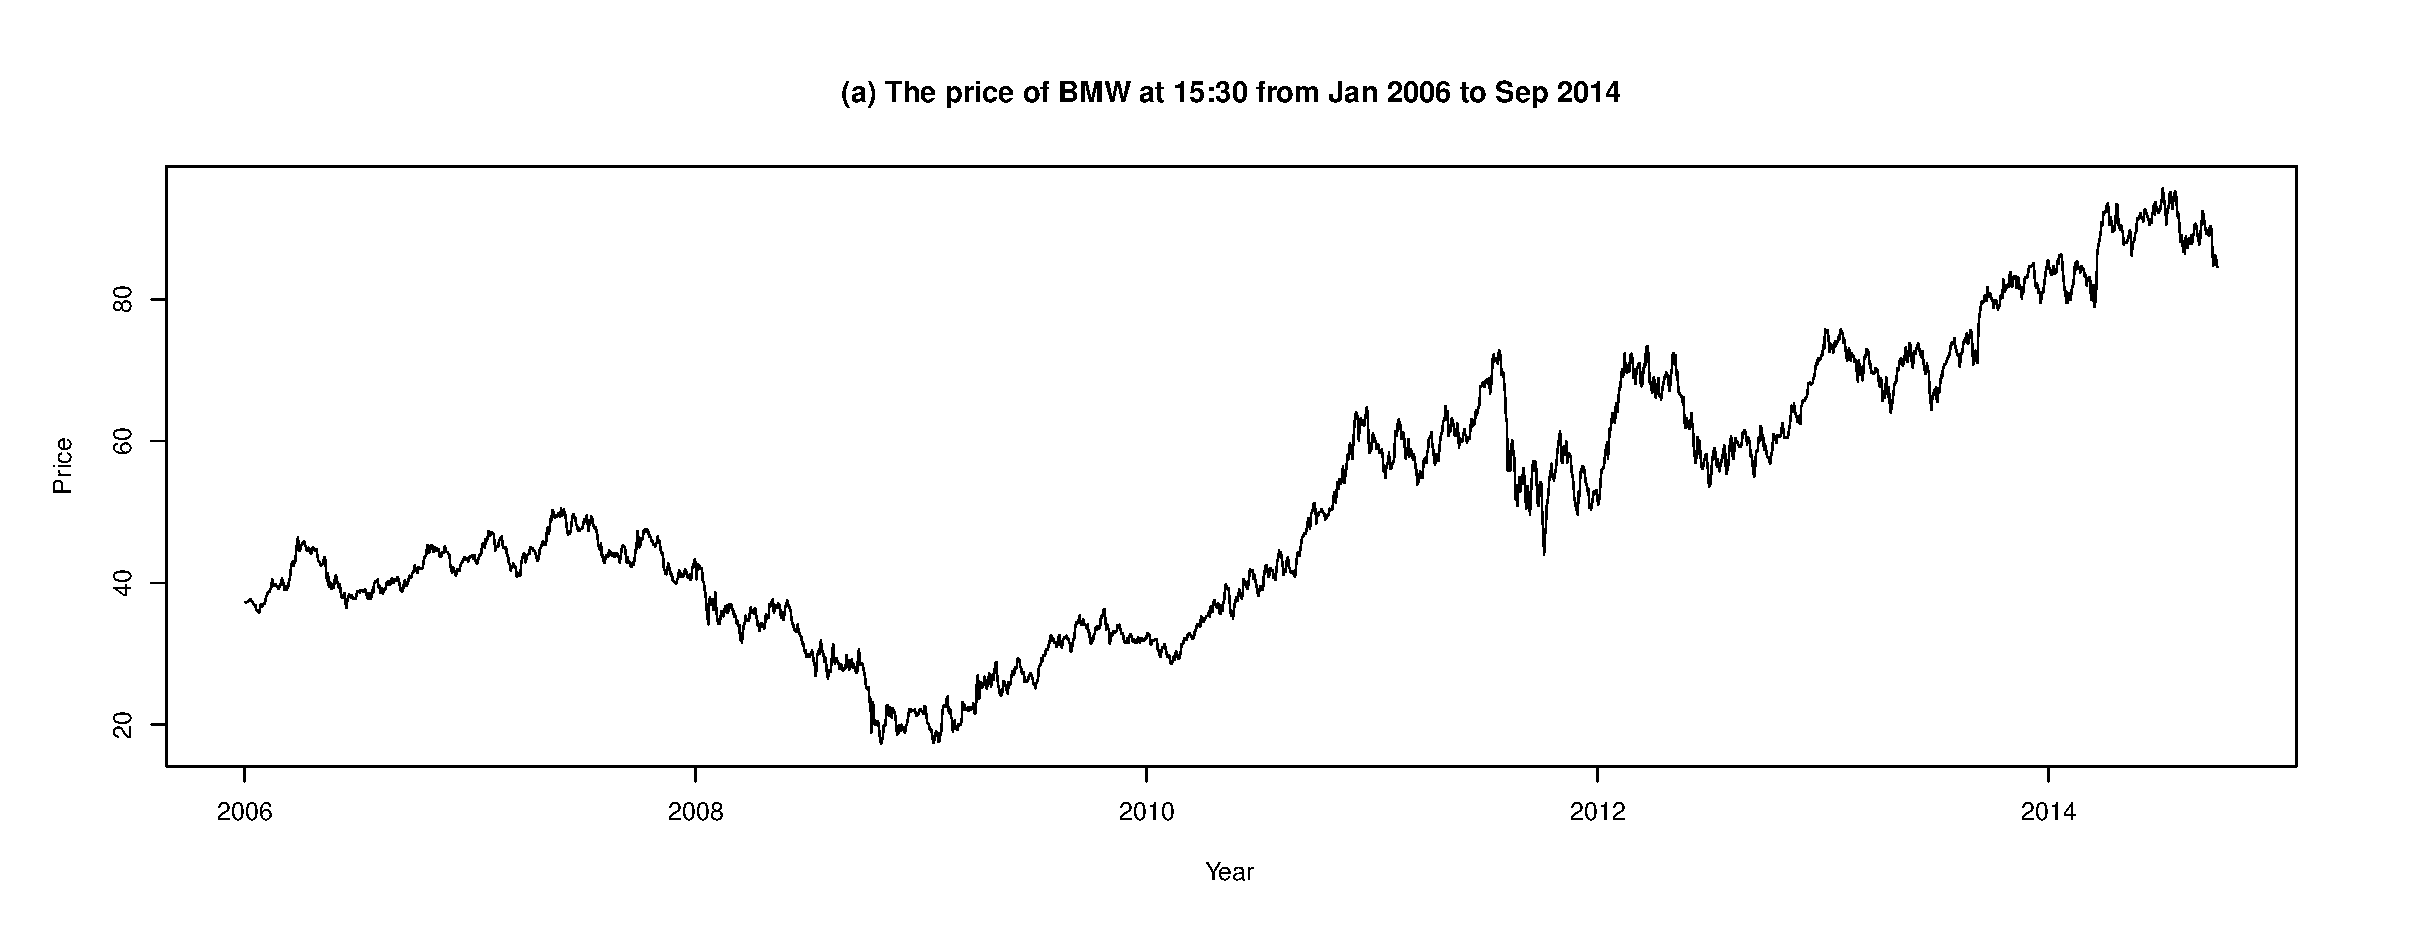
\includegraphics[scale=0.6]{Images/bmw/BMW1530_001.ps}
%%
%%	\label{fig:BMW1530_001}
%%\end{figure}
%
%
%\begin{figure}[t]
%	\centering
%	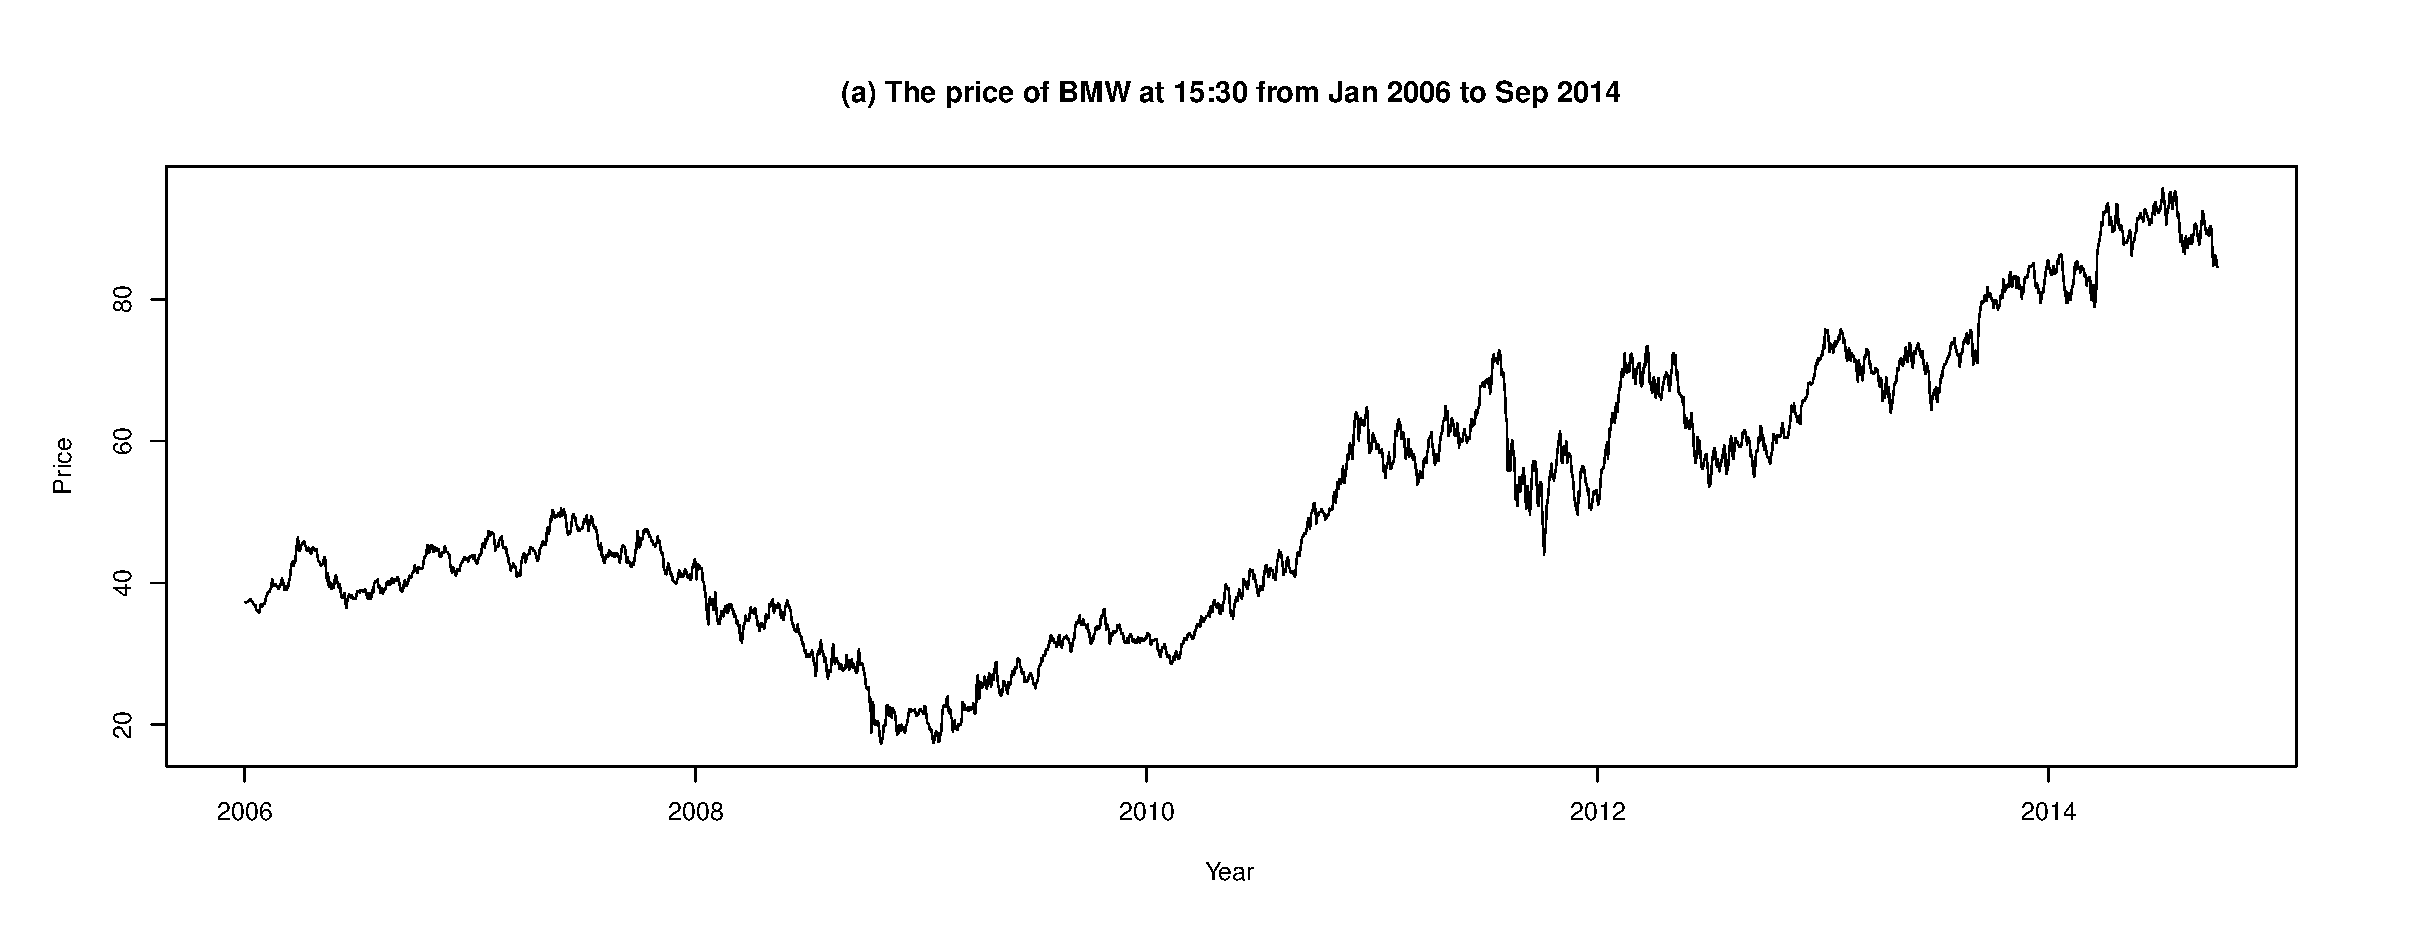
\includegraphics[scale=0.3]{Images/bmw/BMW1530_001}
%	\caption{The price of BMW at 15:30 from Jan 2006 to Sep 2014}
%	\label{fig:BMW1530_001}
%\end{figure}
%
%\begin{figure}[t]
%	\centering
%	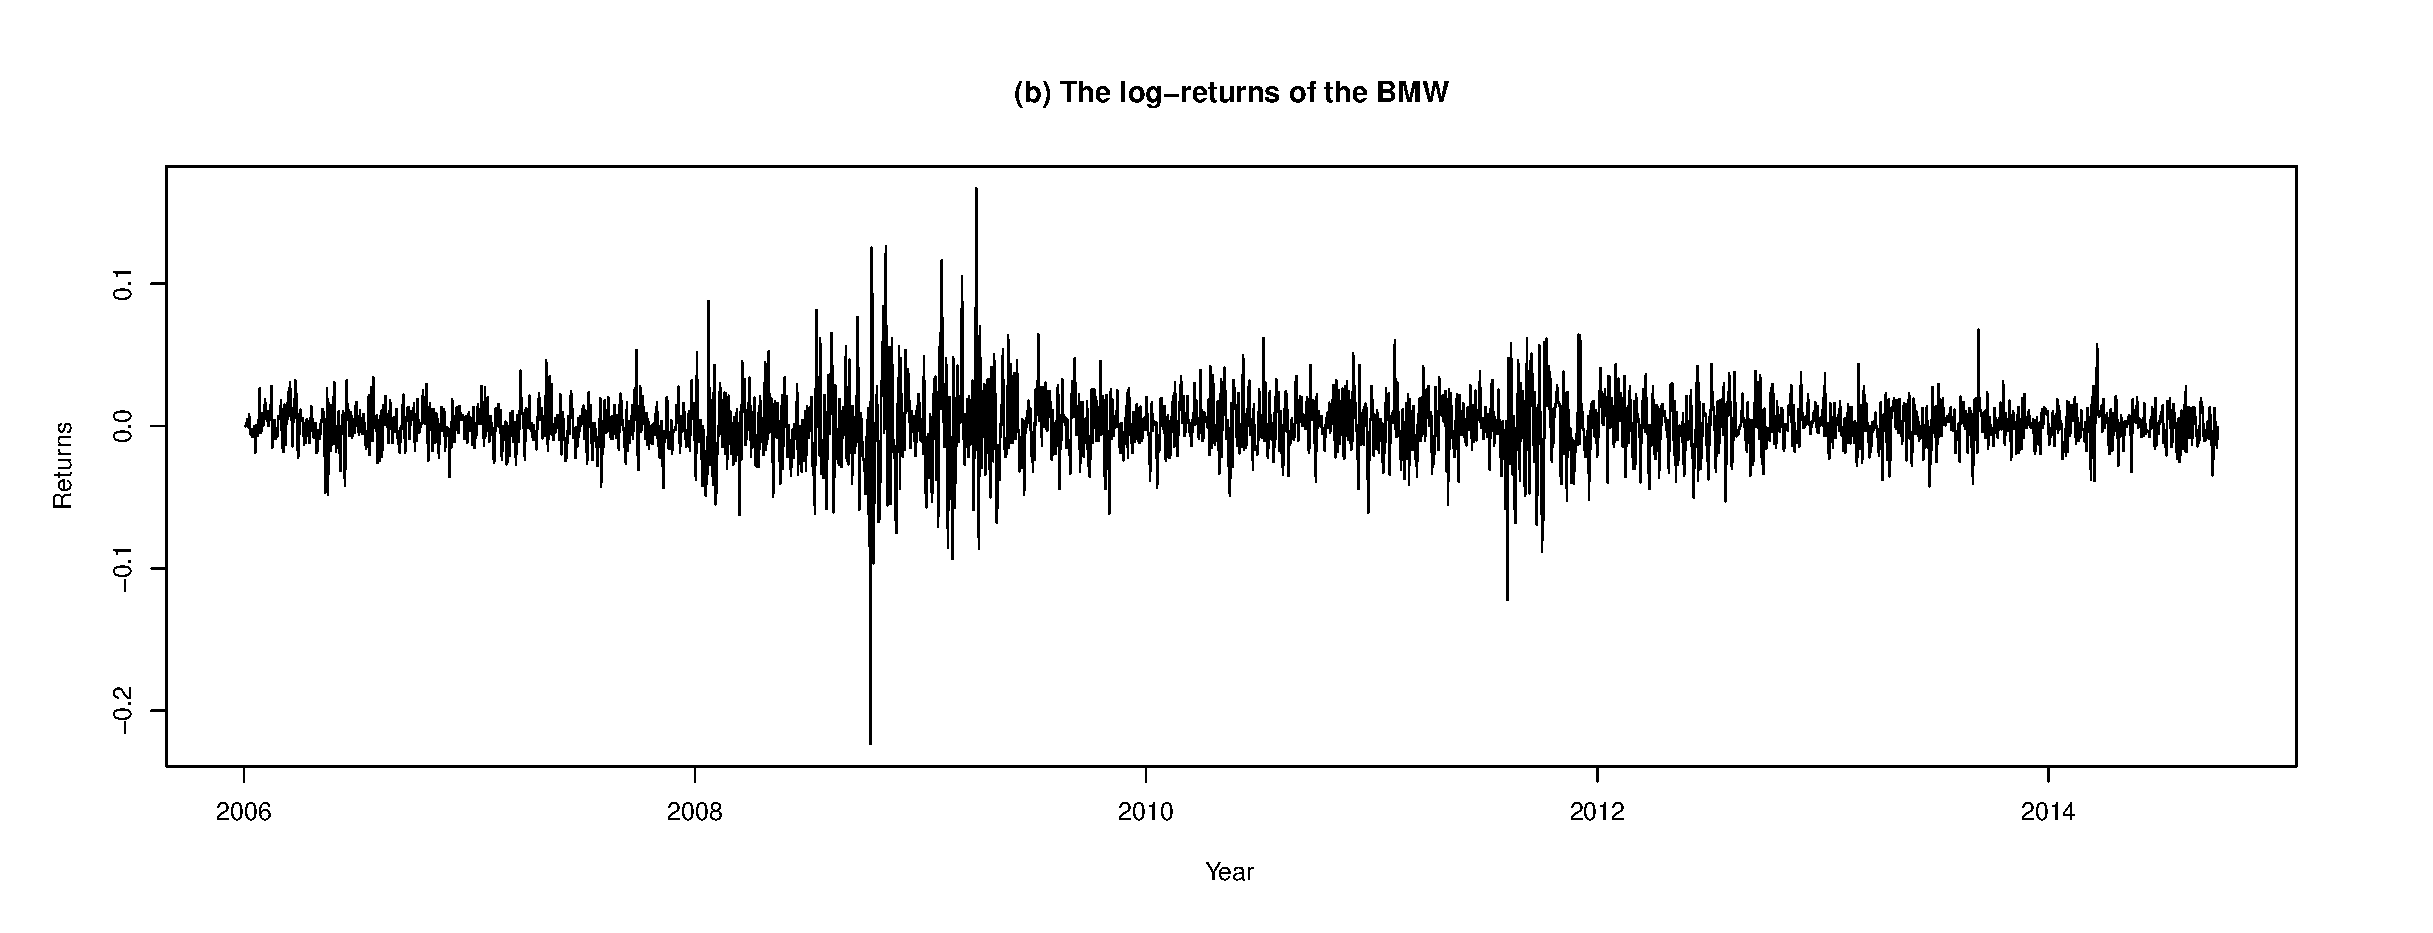
\includegraphics[scale=0.3]{Images/bmw/BMW1530_002}
%	\caption{The log−returns of the BMW}
%	\label{fig:BMW1530_002}
%\end{figure}
%\begin{figure}[t]
%	\centering
%	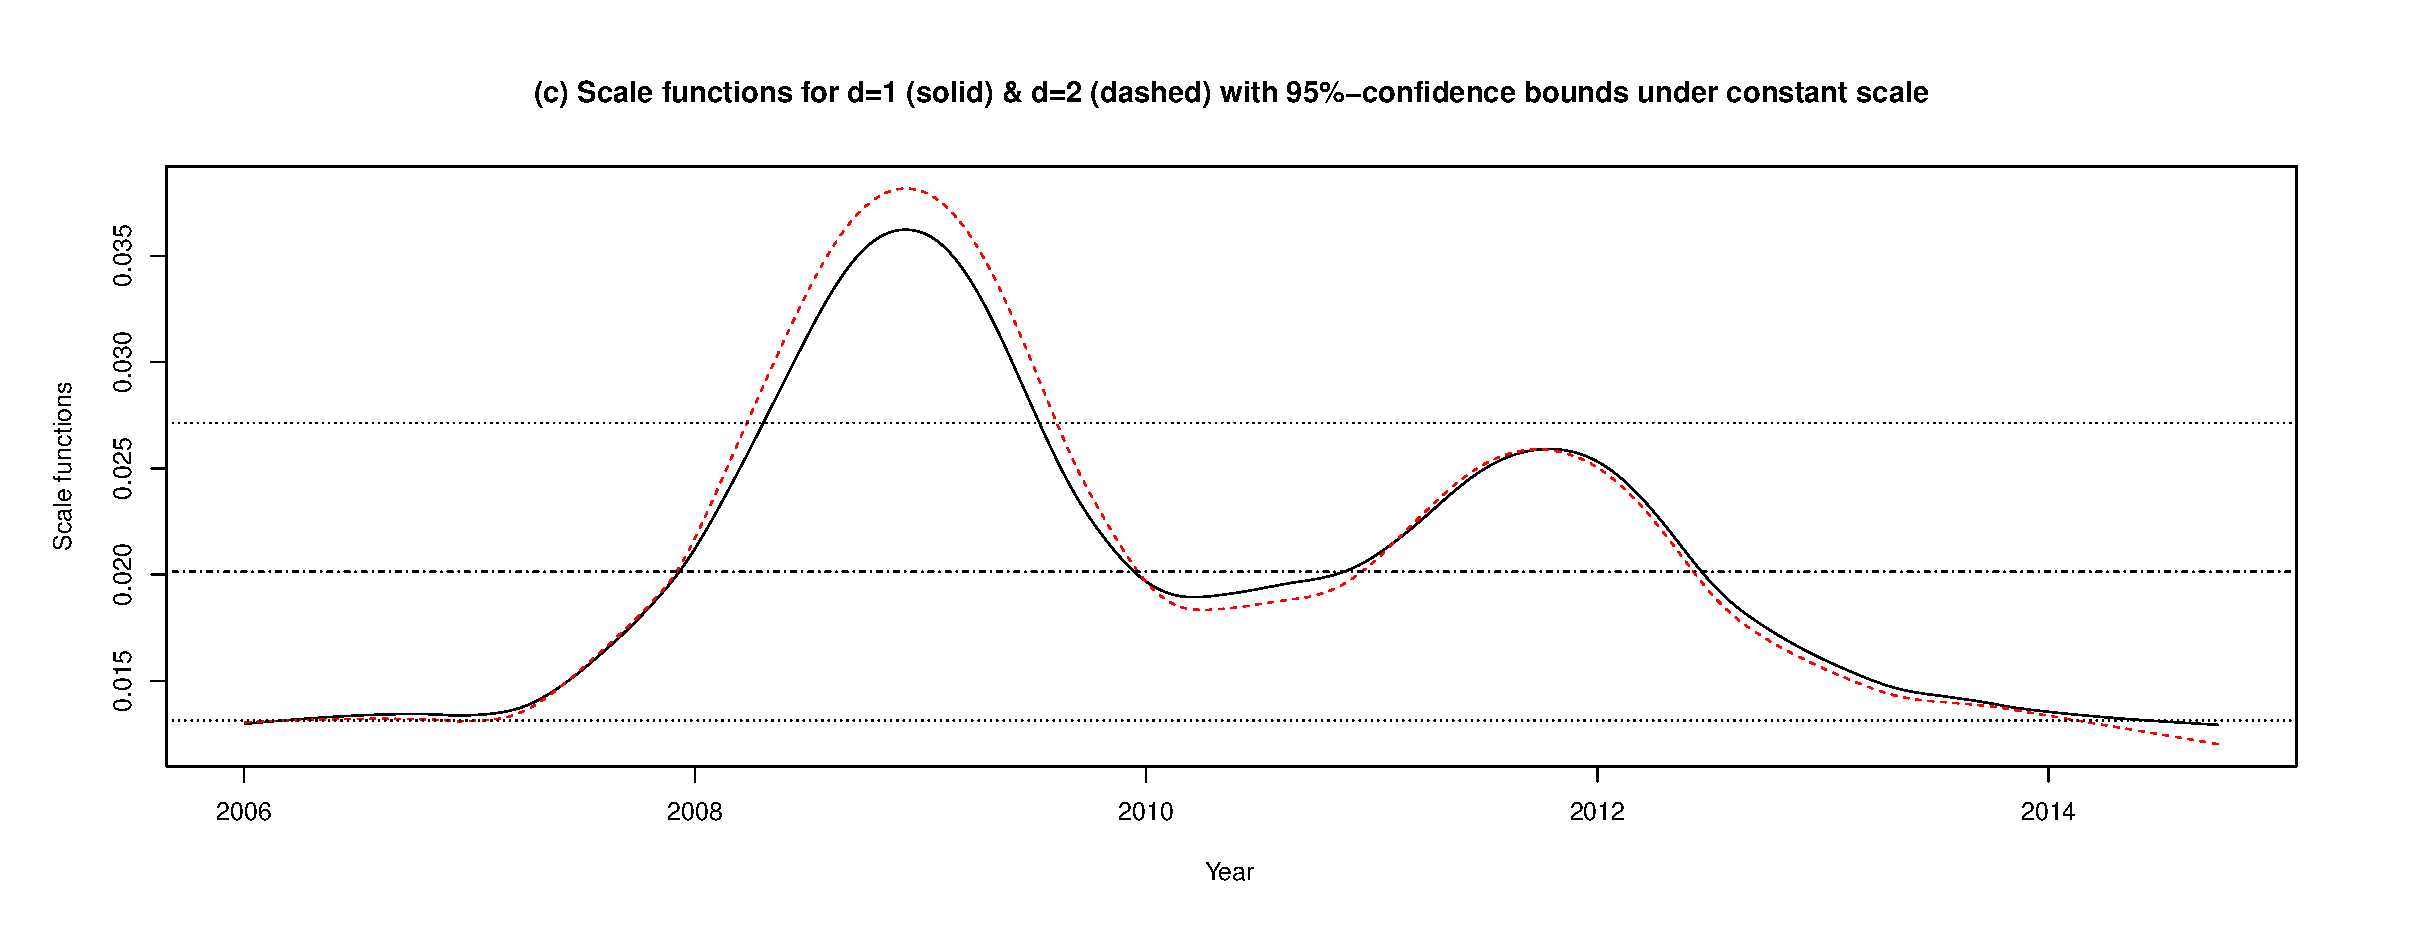
\includegraphics[scale=0.3]{Images/bmw/BMW1530_003}
%	\caption{The price of BMW at 15:30 from Jan 2006 to Sep 2014}
%	\label{fig:BMW1530_003}
%\end{figure}
%\begin{figure}[t]
%	\centering
%	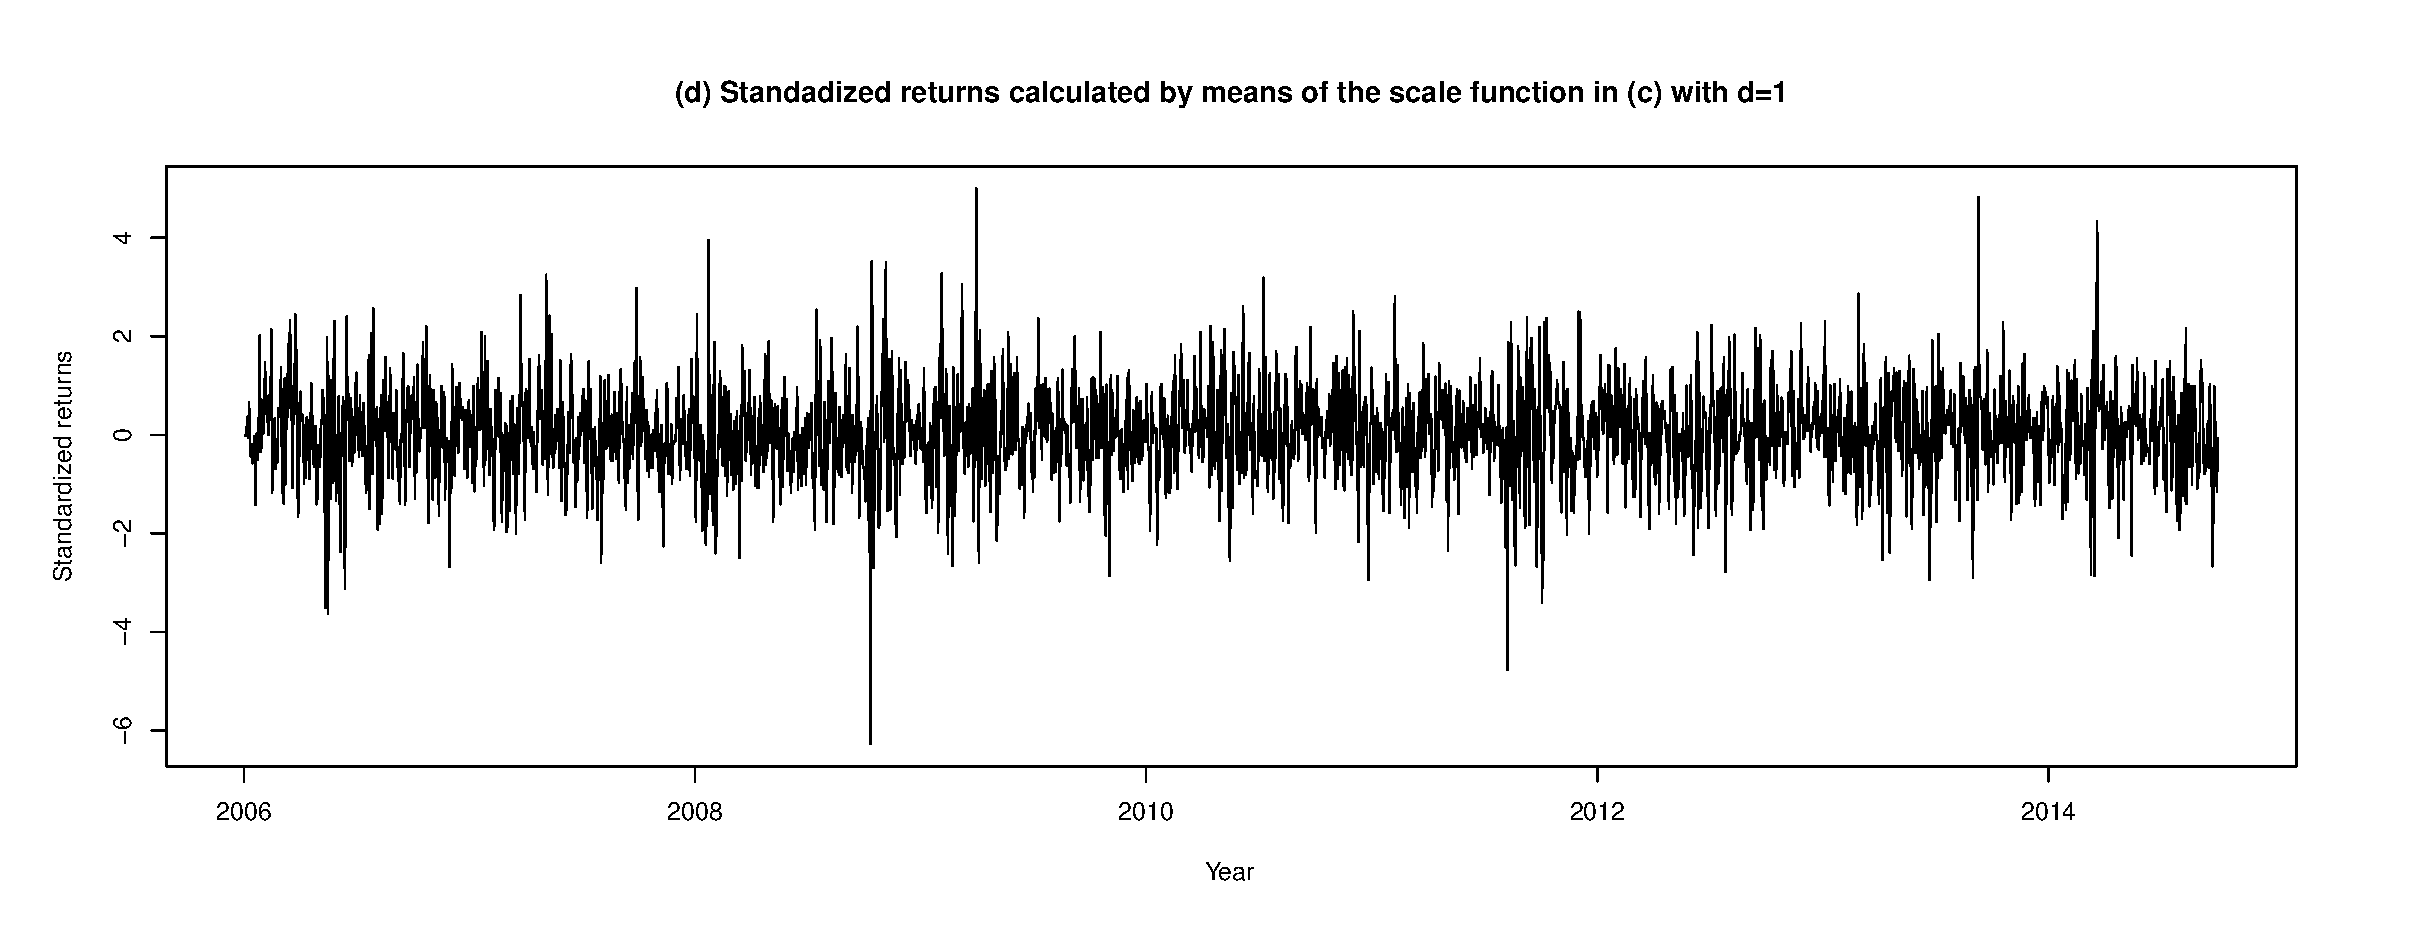
\includegraphics[scale=0.3]{Images/bmw/BMW1530_004}
%	\caption{The price of BMW at 15:30 from Jan 2006 to Sep 2014}
%	\label{fig:BMW1530_004}
%\end{figure}
%
%



%######################## Chapter 4 ######################################################
%\clearemptydoublepage
\chapter{Empirical Example}


\section{Data and Methodology}

In this paper the semi-parametric models are applied to ten sets of high-frequency financial data, which are the stock price of the BMW and the Allianz with five given trading time points from January 2006 to September 2014, respectively. High-frequency financial data are observations of financial variables taken daily or at a finer time scale. Because the high- frequency financial data exhibits the features that has better consistency with the practice, it is more useful for studying the statistical properties and volatility in particular \citep{Zivot2005}.

Usually, in the literatures the daily observations are applied, which are generally composed of the average value or the close price of a trading day. By using these data, the analysis is not accurate enough and the characteristics of the return at the different time points in the day cannot be shown. Therefore, to get the more exact results the observations at five fixed trading time points are selected in this work, i.e. 09:30, 11:00, 12:30, 14:00 and 15:30. In one data set, the neighbor observations are 24 hours apart, which means they are exact daily data. Because of the ``overnight effect'' the open price is not chosen. The ``overnight effect'' means that, the open price may be obviously different from the price at other time points. Normally, the government selects to release the important issues after the stock markets closed, in order to avoid that the investors cannot immediately reflect to the information. This may cause irrational fluctuations of the stock price at open. Furthermore, because of the time difference, the abroad information may also cause an abnormal fluctuation of open price \citep{Tsai2012}. Sometimes, in order to avoid this potential risk, the stockholders choose to change their equity of stock holding at the close time, which may result in the abnormal fluctuation of close price. Therefore, the close price is also excluded. 

In the empirical examples, the characters of the semi-parametric models, the comparison between the semi-parametric models and the parametric models, the volatility of returns at the different trading times in one day and influence of the financial crisis on the companies will be shown by analyzing the empirical results. To deal with the data and get the fitted models, R, a free and open sourced statistics and econometrics software, is used. It is easy to use and the package of R will extend with the development of the model. Many new products in the statistics were originally appeared as a R package before became a business platform, e.g. the ``fgarch'' and ``rugarch'' package, which will be used for data processing in this work \citep{Consulting2013}.

Firstly, the fitted scale function of semi-parametric is estimated by using the ``fgarch'' package of R. The applied method was discussed in semi-parametric APARCH model as mentioned above. Here the bandwidth is selected automatically by R \citep{Wuertz2013}. An initial bandwidth is given according to Cross-Validation. Then the final best bandwidth is selected by the plug-in method. Secondly, the standardized returns are obtained by the means of the estimated scale function. Thirdly, the fitted semi-parametric APARCH, EGARCH and CGARCH models of the orders (1,1), (1,2), (2,1) and (2,2) are got by using the ``rugarch'' package of R
 \citep{Ghalanos2014a}.In these processes, the distribution is assumed as the student-t distribution. The t distribution has fatter tails and is more leptokurtic than normal distribution \citep{Pollard1998}. From table \ref{tab:table-stu-alc} we can also see that, the models with student-t distribution have smaller Bayesian information criterion (BIC) than the ones with normal distribution. BIC is a criterion for model selection. The lower the BIC, the better the model \citep{Schwarz1978}. Furthermore, by using student-t distribution, an additional parameter ``shape'' can be under consideration, which expresses the degrees of freedom and can help to discuss the existence of the conditional variance’s 2mth moment and the development level of the company. Finally, the best semi-parametric model will be selected through comparing the BIC. Then the risk and the leverage effect can be discussed by the empirical results.

\begin{table}[!h]
  \small
  \centering
  \vspace{2ex}
%\resizebox{\textwidth}{!}{ % compress table
\begin{tabular}{c|cc|cc|cc}
\toprule
\multirow{2}{*}{} &
\multicolumn{2}{c|}{APARCH(1,1)} &
\multicolumn{2}{c|}{EGARCH(1,1)} &
\multicolumn{2}{c}{CGARCH(1,1)} \\
\cline{1-3}\cline{4-5}\cline{6-7}
& norm  & std & norm  & std & norm   & std  \\
\midrule
\hline
T = 09:30  & 2.7459 & 2.7117 & 2.7473 & 2.7108 & 2.7689 & 2.7283 \\

T = 11:00  & 2.7816 & 2.7542 & 2.7815 & 2.7528 & 2.7996 & 2.7671 \\

T = 12:30  & 2.7828 & 2.7543 & 2.7826 & 2.7524 & 2.8041 & 2.7690 \\

T = 14:00  & 2.7738 & 2.7424 & 2.7713 & 2.7396 & 2.8001 & 2.7592 \\

T = 15:30  & 2.7921 & 2.7558 & 2.7923 & 2.7545 & 2.8084 & 2.7715 \\

\bottomrule


\end{tabular}
%} %end of compress

  \caption{BIC of selected models with normal and student-t distribution for Alianz}
  \label{tab:table-stu-alc}
  
\end{table}

%\section{Semi-parametric application in Allianz}
\section{Empirical Result of Allianz}

At first, the proposed algorithm is applied to the returns of Allianz at five given trading time points. The long-term risks of these five data sets are analyzed through the estimated scale function; the short-term risks and the leverage effect are estimated by discussing the conditional heteroskedasticity by using APARCH, EGARCH and CGARCH models of a best order based on standardized returns. 

\subsection{Analysis of the long-term risk}


There are four plots in figure \ref{fig:ALV0930}, \ref{fig:ALV1100}, \ref{fig:ALV1230}, \ref{fig:ALV1400} and \ref{fig:ALV1530}, respectively: the observations, the returns series, the estimated scale functions with d=1(solid line) and d=2(dashed line), and the standardized returns, which is calculated by means of the estimated scale function in (c) with d=1. 
According to the plots (b), the return series show up two times strong volatilities. The first one is the financial crisis in 2007/2008. The American subprime loan defaults soar caused the shock, fear and crisis in the international financial market in 2007 and spread to a global financial crisis in 2008. The second one is the ``Euro crisis'', which happened in August and September 2011. The global financial crisis in 2008 caused serious negative influences for the economy in many European countries. In order to save the bank, the sovereign debt increased sharply and exceeded the solvency in several countries. This crisis started from the Greece debt crisis in 2010, and nearly the whole Europe was involved in until September 2011. The high peaks of scale function show that, this company has extremely high long-term risk during the financial crisis. From these figures, it also can be seen that the volatility at 09:30 is strongest in all the given trading time points because of the ``overnight effect''. 

From the plots(c) we can see that, corresponding the volatility of returns, there are two sub-periods of the scale function with high peaks during the two financial crises; and the first peak is higher than the second one, which indicates that the company Allianz had higher risk during the financial crisis 2007/2008 than the ``Euro crisis''.

\begin{figure}[!htbp]
	\centering
	\includegraphics[width=\textwidth]{Images/alv/ALV0930}
	\caption[The smoothing results for ALV at 09:30]{The smoothing results for ALV at 09:30}
	\label{fig:ALV0930}
\end{figure}


\begin{figure}[!htbp]
	\centering
	\includegraphics[width=\textwidth]{Images/alv/ALV1100}
	\caption[The smoothing results for ALV at 11:00]{The smoothing results for ALV at 11:00}
	\label{fig:ALV1100}
\end{figure}

\begin{figure}[!htbp]
	\centering
	\includegraphics[width=\textwidth]{Images/alv/ALV1230}
	\caption[The smoothing results for ALV at 12:30]{The smoothing results for ALV at 12:30}
	\label{fig:ALV1230}
\end{figure}

\begin{figure}[!htbp]
	\centering
	\includegraphics[width=\textwidth]{Images/alv/ALV1400}
	\caption[The smoothing results for ALV at 14:00]{The smoothing results for ALV at 14:00}
	\label{fig:ALV1400}
\end{figure}

\begin{figure}[!htbp]
	\centering
	\includegraphics[width=\textwidth]{Images/alv/ALV1530}
	\caption[The smoothing results for ALV at 15:30]{The smoothing results for ALV at 15:30}
	\label{fig:ALV1530}
\end{figure}

Except the two financial crises, the scale functions stay at a relatively low level in the whole selected time area, usually in the below area of the confidence interval. This means that the financial market developed stable in these periods. However, the stock prices in the time between the two financial crises stay at a relatively low level. From this we can know that, the negative influence of the global financial crisis in 2007/2008 cannot be totally compensated before the second financial crisis started. 

Comparing the scale functions for the given trading time points, which are estimated with d=1 and d=2, we can see that they are generally the same in the stable periods. The differences between the two estimated scale functions often appeared at the boundary or during the financial crisis. For example, the estimated scale functions at 12:30 and 14:00 with d=1 are below the ones with d=2 at the outbreak of the two financial crises, and are clearly up at the beginning of the crises. 
Furthermore, the estimated scale functions at 09:30, 11:00 and 15:30 show up more differences between with d=1 and d=2. The scale function with d=1 at 09:30 is clearly up the one with d=2 at the beginning of the global financial crisis in 2007/2008. Then the increasing speed of the scale function with d=1 becomes gradually slow. In the worst several months of the financial crisis the scale function with d=1 stays below the one with d=2. In the ``Euro crisis'', the scale function with d=1 is also up the one with d=2 at the beginning; and then the two lines tend to be overlapped. At 11:00 and 15:30, the differences between the scale functions with d=1 and d=2 are more obvious. The scale function with d=1 is clearly up the one with d=2 at the beginning of each financial crisis. When the scale functions reach to the highest level, the scale function with d=1 stays at a significant lower level than the one with d=2. Then it becomes higher than d=2 again as the decline of the financial crisis.

According to above discussion, the following standardized returns are calculated by using the scale function with d=1. Firstly, the selected bandwidths for d=1 are generally smaller than that for d=2(table \ref{tab:bandwidthALV}). Generally speaking, the smaller bandwidth is preferred. Secondly, when the scale function with d=1 is applied, the returns are estimated by the absolute returns. In this case, only the existence of fourth moment of conditional variance should be required. However, with the scale function with d=2 the returns are estimated by the square returns. The conditional variance's eighth moment should be exist. From the above discussion, the eighth moment of conditional variance in most cases does not exist. Furthermore, by using d=1 the boundary problem can be solved, while this may cause an abnormal fluctuation with d=2.


%%%%%%%%%%%%%%%%%%%%%%%%%%%%%%%%%%%%%%%%%%%%%%%%%%%%%%
% Begin of Table Selected bandwidths in all times(T) of ALV
%%%%%%%%%%%%%%%%%%%%%%%%%%%%%%%%%%%%%%%%%%%%%%%%%%%%%%
\begin{table}[!h]
 \small
  \centering
  \vspace{2ex} 
\begin{tabular}{c|c|c|c|c|c}
\toprule
    &T=09:30&T=11:00&T=12:30&T=14:00&T=15:30 \\
\midrule
\hline
d=1	&0.09845639	& 0.0932583		&0.09118069	& 0.09206592  &	0.1017511\\
d=2	&0.1069041	& 0.1046261		&0.09312175	& 0.1070296	  &   0.08780973\\
\bottomrule

\end{tabular}
  \caption{Selected bandwidths in all times(T) of ALV}
  \label{tab:bandwidthALV}
\end{table}

%%%%%%%%%%%%%%%%%%%%%%%%%%%%%%%%%%%%%%%%%%%%%%%%%%%%%%
% End of Table Selected bandwidths in all times(T) of ALV
%%%%%%%%%%%%%%%%%%%%%%%%%%%%%%%%%%%%%%%%%%%%%%%%%%%%%%



\subsection{Analysis of the conditional behaviors}

According to plots (d), the standardized return series are quite stable. However, because the nonparametric and parametric components are almost orthogonal to each other, the series still clearly exhibit the influence of market changes that is not affected by estimating or removing the nonparametric component.

By using the ``rugarch'' package in R the fitted APACH, EGARCH and CGARCH models of orders (1,1), (1,2), (2,1) and (2,2) under the student-t distribution can be obtained based on the standardized returns. The best order in all cases is the order (1,1) through comparing the BIC in table \ref{tab:bicALV}. Therefore, we only discuss APARCH(1,1), EGARCH(1,1) and CGARCH(1,1) models in this work.



%%%%%%%%%%%%%%%%%%%%%%%%%%%%%%%%%%%%%%%%%%%%%%%%%%%%%%%%%%%%%%%%%%%%%%%%%%%%%%%%
% Begin of BIC of all selected models for ALV
%%%%%%%%%%%%%%%%%%%%%%%%%%%%%%%%%%%%%%%%%%%%%%%%%%%%%%%%%%%%%%%%%%%%%%%%%%%%%%%%

\begin{table}[!h]
 \small
  \centering
  \vspace{2ex} 
\begin{tabular}{c|c|c|c|c|c}
\toprule
	         &	T=09:30	&T=11:00&T=12:30&T=14:00&T=15:30\\
\midrule
\hline		 

APARCH-t(1,1)&	2.7117	&2.7542	&2.7543	&2.7424	&2.7558 \\

APARCH-t(1,2)&	2.7151	&2.7577	&2.7577	&2.7458	&2.7593 \\

APARCH-t(2,1)&	2.7183	&2.7611	&2.7606	&2.7493	&2.7622 \\

APARCH-t(2,2)&	2.7218	&2.7645	&2.7641	&2.7524	&2.7656 \\

EGARCH-t(1,1)&	2.7108	&2.7528	&2.7524	&2.7396	&2.7545 \\

EGARCH-t(1,2)&	2.7142	&2.7562	&2.7558	&2.7430	&2.7580 \\

EGARCH-t(2,1)&	2.7176	&2.7597	&2.7579	&2.7458	&2.7609 \\

EGARCH-t(2,2)&	2.7204	&2.7631	&2.7614	&2.7492	&2.7646 \\

CGARCH-t(1,1)&	2.7283&	2.7671&	2.7690	&2.7592	&2.7715 \\

CGARCH-t(1,2)&	2.7309&	2.7706&	2.7725	&2.7627	&2.7750\\

CGARCH-t(2,1)&	2.7317&	2.7706&	2.7721	&2.7625	&2.7742\\

CGARCH-t(2,2)&	2.7342&	2.7740&	2.7756	&2.7660	&2.7777\\

\bottomrule

\end{tabular}
  \caption{BIC of all selected models for ALV}
  \label{tab:bicALV}
\end{table}
%%%%%%%%%%%%%%%%%%%%%%%%%%%%%%%%%%%%%%%%%%%%%%%%%%%%%%%%%%%%%%%%%%%%%%%%%%%%%%%%
% End of BIC of all selected models for ALV
%%%%%%%%%%%%%%%%%%%%%%%%%%%%%%%%%%%%%%%%%%%%%%%%%%%%%%%%%%%%%%%%%%%%%%%%%%%%%%%%


%%%%%%%%%%%%%%%%%%%%%%%%%%%%%%%%%%%%%%%%%%%%%%%%%%%%%%%%%%%%%%%%%%%%%%%%%%%%%%%%
% Begin of Table Estimated coefficients of the Selected models for ALV at 9:30
%%%%%%%%%%%%%%%%%%%%%%%%%%%%%%%%%%%%%%%%%%%%%%%%%%%%%%%%%%%%%%%%%%%%%%%%%%%%%%%%

\begin{table}[!h]
 \small
  \centering
  \vspace{2ex}

%\resizebox{\textwidth}{!}{ % compress table
  
\begin{tabular}{c|cc|cc|cc}
\toprule
\multirow{2}{*}{} &
\multicolumn{2}{c|}{APARCH(1,1)} &
\multicolumn{2}{c|}{EGARCH(1,1)} &
\multicolumn{2}{c} {CGARCH(1,1)} \\
\cline{1-3}\cline{4-5}\cline{6-7}

& Coeff  & s.e. & Coeff  & s.e. & Coeff   & s.e.  \\
\midrule
\hline
$\mu$       & 0.0308 & 0.0182	& 0.0235	& 0.0181  & 0.0462  & 0.0180    \\
$\omega$    & 0.0721 & 0.0172	& -0.0085	& 0.0060  & 0.0047  & 0.0006    \\
$\alpha_1$  & 0.0656 & 0.0309	& -0.1215	& 0.0208  & 0.1018  & 0.0191    \\
$\beta_1$   & 0.8411 & 0.0288	& 0.9281	& 0.0167  & 0.8351  & 0.0300    \\
$\gamma_1 $ & 0.7207 & 0.3454	& 0.1729	& 0.0304  & -		& -			\\
$\delta$    & 1.8156 & 0.3597	& -			& -		  & -		& -			\\
$\eta_{11}$ & -	 	 & -     	& -			& - 	  & 0.9956 	& 0.0000	\\
$\eta_{21}$ & -		 & -     	& -			& - 	  & 0.0000 	& 0.0000	\\
shape       & 6.5064 & 0.8851	& 6.3915	& 0.8530  & 6.0607 	& 0.7792	\\

% $\alpha_2$   & - & - & - & - & 0.021706 & 0.011395 \\

%$\gamma_2$   & - & - & - & - &1 \\

%$\beta_1$  &  & &0.00000001&0.08676& - & -\\

%$\sigma_1$ & 1.017673 & 0.12041 & 1.01704876 & 0.1207 & 1.058141 & 0.127632 \\

\bottomrule
\end{tabular}
%} %end of compress
  \caption{Estimated coefficients of the Selected models at 09:30 for ALV}
  \label{tab:coefALV930}

\end{table}

%%%%%%%%%%%%%%%%%%%%%%%%%%%%%%%%%%%%%%%%%%%%%%%%%%%%%%%%%%%%%%%%%%%%%%%%%%%%%%%%
% End of Table Estimated coefficients of the Selected models for ALV at 9:30
%%%%%%%%%%%%%%%%%%%%%%%%%%%%%%%%%%%%%%%%%%%%%%%%%%%%%%%%%%%%%%%%%%%%%%%%%%%%%%%%



%%%%%%%%%%%%%%%%%%%%%%%%%%%%%%%%%%%%%%%%%%%%%%%%%%%%%%%%%%%%%%%%%%%%%%%%%%%%%%%%
% Begin of Table Estimated coefficients of the Selected models for ALV at 11:00
%%%%%%%%%%%%%%%%%%%%%%%%%%%%%%%%%%%%%%%%%%%%%%%%%%%%%%%%%%%%%%%%%%%%%%%%%%%%%%%%

\begin{table}[!h]
 \small
  \centering
  \vspace{2ex}

%\resizebox{\textwidth}{!}{ % compress table
  
\begin{tabular}{c|cc|cc|cc}
\toprule
\multirow{2}{*}{} &
\multicolumn{2}{c|}{APARCH(1,1)} &
\multicolumn{2}{c|}{EGARCH(1,1)} &
\multicolumn{2}{c} {CGARCH(1,1)} \\
\cline{1-3}\cline{4-5}\cline{6-7}

& Coeff  & s.e. & Coeff  & s.e. & Coeff   & s.e.  \\
\midrule
\hline

$\mu$       & 0.0279	& 0.0189	& 0.0282	& 0.0191  & 0.0442	& 0.0187    \\
$\omega$    & 0.0868	& 0.0219	& -0.0068	& 0.0059  & 0.0054	& 0.0006    \\
$\alpha_1$  & 0.0717	& 0.0226	& -0.1202	& 0.0215  & 0.0915	& 0.0188    \\
$\beta_1$   & 0.8336	& 0.0341	& 0.9160	& 0.0210  & 0.8412	& 0.0347    \\
$\gamma_1 $ & 0.6554	& 0.2800	& 0.1427	& 0.0304  & -     	& -     	\\
$\delta$    & 1.6610	& 0.3892	& -     	& -       & -     	& -     	\\
$\eta_{11}$ & -     	& -     	& -     	& -       & 0.9949	& 0.0000	\\
$\eta_{21}$ & -     	& -     	& -    		& -       & 0.0000	& 0.0000	\\
shape       & 7.3037	& 1.1341	& 7.1364	& 1.0881  & 6.9448	& 1.0259	\\

\bottomrule
\end{tabular}
%} %end of compress
  \caption{Estimated coefficients of the Selected models at 11:00 for ALV}
  \label{tab:coefALV1100}

\end{table}

%%%%%%%%%%%%%%%%%%%%%%%%%%%%%%%%%%%%%%%%%%%%%%%%%%%%%%%%%%%%%%%%%%%%%%%%%%%%%%%%
% End of Table Estimated coefficients of the Selected models for ALV at 11:00
%%%%%%%%%%%%%%%%%%%%%%%%%%%%%%%%%%%%%%%%%%%%%%%%%%%%%%%%%%%%%%%%%%%%%%%%%%%%%%%%



%%%%%%%%%%%%%%%%%%%%%%%%%%%%%%%%%%%%%%%%%%%%%%%%%%%%%%%%%%%%%%%%%%%%%%%%%%%%%%%%
% Begin of Table Estimated coefficients of the Selected models for ALV at 12:30
%%%%%%%%%%%%%%%%%%%%%%%%%%%%%%%%%%%%%%%%%%%%%%%%%%%%%%%%%%%%%%%%%%%%%%%%%%%%%%%%

\begin{table}[!h]
 \small
  \centering
  \vspace{2ex}

%\resizebox{\textwidth}{!}{ % compress table
  
\begin{tabular}{c|cc|cc|cc}
\toprule
\multirow{2}{*}{} &
\multicolumn{2}{c|}{APARCH(1,1)} &
\multicolumn{2}{c|}{EGARCH(1,1)} &
\multicolumn{2}{c} {CGARCH(1,1)} \\
\cline{1-3}\cline{4-5}\cline{6-7}

& Coeff  & s.e. & Coeff  & s.e. & Coeff   & s.e.  \\
\midrule
\hline

$\mu$       & 0.0242	& 0.0190	& 0.0201	& 0.0190	& 0.0438	& 0.0188    \\
$\omega$    & 0.0858	& 0.0204	&-0.0068	& 0.0057	& 0.0034	& 0.0003    \\
$\alpha_1$  & 0.0724	& 0.0215	&-0.1192	& 0.0208	& 0.0921	& 0.0181    \\
$\beta_1$   & 0.8398	& 0.0311	& 0.9174	& 0.0200	& 0.8330	& 0.0324    \\
$\gamma_1 $ & 0.7439	& 0.2797	& 0.1439	& 0.0307	& -     	& -     	\\
$\delta$    & 1.4690	& 0.2978	& -     	& -     	& -     	& -     	\\
$\eta_{11}$ & -     	& -     	& -     	& -     	& 0.9967	& 0.0000	\\
$\eta_{21}$ & -     	& -     	& -     	& -     	& 0.0000	& 0.0000	\\
shape       & 7.9157	& 1.2338	& 7.7971	& 1.1984	& 7.2398	& 1.0469	\\

\bottomrule
\end{tabular}
%} %end of compress
  \caption{Estimated coefficients of the Selected models at 12:30 for ALV}
  \label{tab:coefALV1230}

\end{table}

%%%%%%%%%%%%%%%%%%%%%%%%%%%%%%%%%%%%%%%%%%%%%%%%%%%%%%%%%%%%%%%%%%%%%%%%%%%%%%%%
% End of Table Estimated coefficients of the Selected models for ALV at 12:30
%%%%%%%%%%%%%%%%%%%%%%%%%%%%%%%%%%%%%%%%%%%%%%%%%%%%%%%%%%%%%%%%%%%%%%%%%%%%%%%%



%%%%%%%%%%%%%%%%%%%%%%%%%%%%%%%%%%%%%%%%%%%%%%%%%%%%%%%%%%%%%%%%%%%%%%%%%%%%%%%%
% Begin of Table Estimated coefficients of the Selected models for ALV at 14:00
%%%%%%%%%%%%%%%%%%%%%%%%%%%%%%%%%%%%%%%%%%%%%%%%%%%%%%%%%%%%%%%%%%%%%%%%%%%%%%%%

\begin{table}[!h]
 \small
  \centering
  \vspace{2ex}

%\resizebox{\textwidth}{!}{ % compress table
  
\begin{tabular}{c|cc|cc|cc}
\toprule
\multirow{2}{*}{} &
\multicolumn{2}{c|}{APARCH(1,1)} &
\multicolumn{2}{c|}{EGARCH(1,1)} &
\multicolumn{2}{c} {CGARCH(1,1)} \\
\cline{1-3}\cline{4-5}\cline{6-7}

& Coeff  & s.e. & Coeff  & s.e. & Coeff   & s.e.  \\
\midrule
\hline

$\mu$       & 0.0237	& 0.0187	&  0.0231	& 0.0180	& 0.0428	& 0.0186    \\
$\omega$    & 0.0957	& 0.0204	& -0.0094	& 0.0067	& 0.0038	& 0.0004    \\
$\alpha_1$  & 0.0884	& 0.0199	& -0.1339	& 0.0220	& 0.1000	& 0.0191    \\
$\beta_1$   & 0.8292	& 0.0291	&  0.9039	& 0.0210	& 0.8207	& 0.0327    \\
$\gamma_1 $ & 0.8207	& 0.2096	&  0.1647	& 0.0324	&  -    	& -     	\\
$\delta$    & 1.1473	& 0.2595	& -      	& -     	&  -    	& -     	\\
$\eta_{11}$ & -     	& -     	& -      	& -     	& 0.9963	& 0.0000	\\
$\eta_{21}$ & -     	& -     	& -      	& -     	& 0.0000	& 0.0000	\\
shape       & 7.4317	& 1.0993	&  7.4128	& 1.0943	& 6.8385	& 0.9355	\\

\bottomrule
\end{tabular}
%} %end of compress
  \caption{Estimated coefficients of the Selected models at 14:00 for ALV}
  \label{tab:coefALV1400}

\end{table}

%%%%%%%%%%%%%%%%%%%%%%%%%%%%%%%%%%%%%%%%%%%%%%%%%%%%%%%%%%%%%%%%%%%%%%%%%%%%%%%%
% End of Table Estimated coefficients of the Selected models for ALV at 14:00
%%%%%%%%%%%%%%%%%%%%%%%%%%%%%%%%%%%%%%%%%%%%%%%%%%%%%%%%%%%%%%%%%%%%%%%%%%%%%%%%


%%%%%%%%%%%%%%%%%%%%%%%%%%%%%%%%%%%%%%%%%%%%%%%%%%%%%%%%%%%%%%%%%%%%%%%%%%%%%%%%
% Begin of Table Estimated coefficients of the Selected models for ALV at 15:30
%%%%%%%%%%%%%%%%%%%%%%%%%%%%%%%%%%%%%%%%%%%%%%%%%%%%%%%%%%%%%%%%%%%%%%%%%%%%%%%%

\begin{table}[!h]
 \small
  \centering
  \vspace{2ex}

%\resizebox{\textwidth}{!}{ % compress table
  
\begin{tabular}{c|cc|cc|cc}
\toprule
\multirow{2}{*}{} &
\multicolumn{2}{c|}{APARCH(1,1)} &
\multicolumn{2}{c|}{EGARCH(1,1)} &
\multicolumn{2}{c} {CGARCH(1,1)} \\
\cline{1-3}\cline{4-5}\cline{6-7}

& Coeff  & s.e. & Coeff  & s.e. & Coeff   & s.e.  \\
\midrule
\hline

$\mu$       & 0.0119	& 0.0190	& 0.0085	& 0.0189	& 0.0295	& 0.0190    \\
$\omega$    & 0.0703	& 0.0189	&-0.0052	& 0.0052	& 0.0041	& 0.0004    \\
$\alpha_1$  & 0.0636	& 0.0221	&-0.1108	& 0.0197	& 0.0830	& 0.0173    \\
$\beta_1$   & 0.8570	& 0.0309	& 0.9281	& 0.0192	& 0.8462	& 0.0333    \\
$\gamma_1 $ & 0.6649	& 0.2724	& 0.1378	& 0.0317	&  -    	& -     	\\
$\delta$    & 1.7361	& 0.4075	& -      	& -     	&  -    	& -     	\\
$\eta_{11}$ & -     	& -     	& -      	& -     	& 0.9960	& 0.0000	\\
$\eta_{21}$ & -     	& -     	& -      	& -     	& 0.0000	& 0.0000	\\
shape       & 8.1277	& 1.2303	& 7.9807	& 1.1877	& 7.6925	& 1.1261	\\

\bottomrule
\end{tabular}
%} %end of compress
  \caption{Estimated coefficients of the Selected models at 15:30 for ALV}
  \label{tab:coefALV1530}

\end{table}

%%%%%%%%%%%%%%%%%%%%%%%%%%%%%%%%%%%%%%%%%%%%%%%%%%%%%%%%%%%%%%%%%%%%%%%%%%%%%%%%
% End of Table Estimated coefficients of the Selected models for ALV at 15:30
%%%%%%%%%%%%%%%%%%%%%%%%%%%%%%%%%%%%%%%%%%%%%%%%%%%%%%%%%%%%%%%%%%%%%%%%%%%%%%%%


Tables \ref{tab:coefALV930}, \ref{tab:coefALV1100}, \ref{tab:coefALV1230}, \ref{tab:coefALV1400}, and \ref{tab:coefALV1530} show the estimated coefficients for Allianz at the five given trading time points, respectively. From these tables we can see that, the APARCH model usually has the largest degree of freedom of the innovation distribution in each case, while the CGARCH model has the smallest one. For the time 09:30, 11:00 and 14:00 the degrees of freedom are all between 6 and 7,5; and for the time 12:30 in all models and 15:30 in EGARCH and CGARCH models the degrees of freedom are almost equal to 8. This means that the distributions in these trading time points are nearly heavy-tailed and the eighth moment of conditional variance $\varepsilon_t$ does not exist, but fourth moment. In APARCH model at 15:30 the degree of freedom is 8.13. Now the distribution is also nearly heavy-tailed but the eighth moment of $\varepsilon_t$ exists. We can see that, the possibility of an extreme return at 09:30, 11:00 and 14:00 is higher than that at 12:30 and 15:30.

If the best model is selected only by comparing BIC, we can see from the table \ref{tab:bicALV} that in all five cases EGARCH model is the best model with the smallest BIC while CGARCH model is the worst. However, different models can be used to different economic situations. APARCH and EGARCH models can show the leverage effect; CGARCH model exhibits the persistence of the shock on the long-term and the short-term.

In APARCH model, the leverage parameter $\gamma$ for the five given trading time points are 0.72, 0.83, 0.74, 0.82 and 0.66, respectively. This means that the leverage effect of Allianz is always strong; and the contribution of a negative return on yesterday to today’s volatility is more than the contribution of a positive return. In EGARCH model, $\alpha$ is the sign effect and $\gamma$ is the size effect. According to the tables, the estimated $\alpha$ is smaller than -0.1 in all cases. Because $\alpha$ is significantly below to zero, we can say that this model also expresses the leverage effect. Volatility tends to rise (fall) when returns surprises are negative (positive), and the negative returns can result in larger volatility.

\begin{figure}[!htbp]
	\centering
	\includegraphics[width=\textwidth]{Images/alv/ALV-0930-semi}
	\caption[The volatility series of different models for ALV at 09:30]{The volatility series of different models for ALV at 09:30}
	\label{fig:ALVsemi0930}
\end{figure}

\begin{figure}[!htbp]
	\centering
	\includegraphics[width=\textwidth]{Images/alv/ALV-1100-semi}
	\caption[The volatility series of different models for ALV at 11:00]{The volatility series of different models for ALV at 11:00}
	\label{fig:ALVsemi1100}
\end{figure}

\begin{figure}[!htbp]
	\centering
	\includegraphics[width=\textwidth]{Images/alv/ALV-1230-semi}
	\caption[The volatility series of different models for ALV at 12:30]{The volatility series of different models for ALV at 12:30}
	\label{fig:ALVsemi1230}
\end{figure}

\begin{figure}[!htbp]
	\centering
	\includegraphics[width=\textwidth]{Images/alv/ALV-1400-semi}
	\caption[The volatility series of different models for ALV at 14:00]{The volatility series of different models for ALV at 14:00}
	\label{fig:ALVsemi1400}
\end{figure}

\begin{figure}[!htbp]
	\centering
	\includegraphics[width=\textwidth]{Images/alv/ALV-1530-semi}
	\caption[The volatility series of different models for ALV at 15:30]{The volatility series of different models for ALV at 15:30}
	\label{fig:ALVsemi1530}
\end{figure}


From the estimated coefficients of CGARCH model, all the $\rho$ values are larger than 0.99, and $\varphi$ are equal to 0. So the immediate impact of shocks on the long-run component would be smaller than that on the short-run component. Because the $\rho$ value is close to 1, the shock cannot only cause the change of short-term volatility, but also keep this abnormal volatility in a long term. The value of $(\alpha + \beta)$ is between 0.9 and 1, and $0 < (\alpha + \beta) < \rho <1$ . This indicates that, volatility can reflect the shock immediately and the persistence is long; the impact of volatility on the short-run component will diminish as well but will be more persistent than of the long-run component.

This result we can also see from figures \ref{fig:ALVsemi0930}, \ref{fig:ALVsemi1100}, \ref{fig:ALVsemi1230}, \ref{fig:ALVsemi1400} and \ref{fig:ALVsemi1530}. All of the APARCH, EGARCH and CGARCH model’s volatility can express the financial crisis. However, when there is positive news, APARCH and EGARCH models have a lower volatility than CGARCH, for example, the marked areas by square; and have a higher volatility for negative news, as the marked areas by round. Moreover, the negative news causes larger change than the positive news. The volatility level of APARCH is larger than EGARCH and CGARCH model.

In this example, by using ``rugarch'' package only one volatility curve of CGARCH is obtained; and this volatility cannot show the persistence of the shock on the long-term and the short-term. Therefore, the volatility of CGARCH is used only to show weather the APARCH and EGARCH models can express the leverage effect. Moreover, we can also see from the figures that, at the first several points the trend of CGARCH’s volatility is abnormally high than other models. Because the earlier returns are required, when the first several points are estimated. This may cause the mistaken calculation. Usually, the first dozens of estimated points are not chosen to discuss. In this case, although the abnormal points appear in the volatility, they do not influence the following trend. Therefore, they are ignored.



\subsection{Comparing the models at the given time points and with daily data}

In order to express the advantage of applying the different given trading time points, the estimated results with given trading time points are compared with the estimated results with the normal daily data.

At first, from the returns in figure \ref{fig:ALVdaily} we can see that, the volatility of returns with the daily data is the strongest during the global financial crisis in 2007/2008 and also stronger than that at other given trading time points except 09:30 during the ``Euro crisis''. The trends of the scale functions with the six data sets are similar, which stay extremely higher level during the financial crisis and lower level during the periods of stable development.


Secondly, the conditional heteroskedasticity following different parametric models are compared. According to the calculation of R, the selected bandwidth with d=1 (0.09) is smaller than the one with d=2 (0.11). Therefore, the standardized returns are also calculated by the means of the scale function with d=1 in this case. Based on the standardized returns, the fitted APARCH, EGARCH and CGARCH models of different orders can be obtained. All the models of the order (1,1) have the smallest BIC(Table \ref{tab:dailyBICforALV}).



%%%%%%%%%%%%%%%%%%%%%%%%%%%%%%%%%%%%%%%%%%%%%%%%%%%%%%%%%%%%%%%%%%%%%%%%%%%%%%%%
% Begin of BIC of the fitted models with daily returns for ALV
%%%%%%%%%%%%%%%%%%%%%%%%%%%%%%%%%%%%%%%%%%%%%%%%%%%%%%%%%%%%%%%%%%%%%%%%%%%%%%%%

\begin{table}[!h]
 \small
  \centering
  \vspace{2ex} 
\begin{tabular}{c|c|c|c}
\toprule
	         &	APARCH	& EGARCH	& CGARCH	\\
\midrule
\hline		 

(1,1)&	2.7048	& 2.7019	&2.7284	 \\
(1,2)&	2.7081	& 2.7051	&2.7318	 \\
(2,1)&	2.7112	& 2.7076	&2.7308	 \\
(2,2)&	2.7147	& 2.7110	&2.7343	 \\
\bottomrule

\end{tabular}
  \caption{BIC of the fitted models with daily returns for ALV}
  \label{tab:dailyBICforALV}
\end{table}
%%%%%%%%%%%%%%%%%%%%%%%%%%%%%%%%%%%%%%%%%%%%%%%%%%%%%%%%%%%%%%%%%%%%%%%%%%%%%%%%
% End of BIC of the fitted models with daily returns for ALV
%%%%%%%%%%%%%%%%%%%%%%%%%%%%%%%%%%%%%%%%%%%%%%%%%%%%%%%%%%%%%%%%%%%%%%%%%%%%%%%%



%%%%%%%%%%%%%%%%%%%%%%%%%%%%%%%%%%%%%%%%%%%%%%%%%%%%%%%%%%%%%%%%%%%%%%%%%%%%%%%%
% Begin of Table Estimated coefficients of the Selected models with daily returns for ALV
%%%%%%%%%%%%%%%%%%%%%%%%%%%%%%%%%%%%%%%%%%%%%%%%%%%%%%%%%%%%%%%%%%%%%%%%%%%%%%%%

\begin{table}[!h]
 \small
  \centering
  \vspace{2ex}

%\resizebox{\textwidth}{!}{ % compress table
  
\begin{tabular}{c|cc|cc|cc}
\toprule
\multirow{2}{*}{} &
\multicolumn{2}{c|}{APARCH(1,1)} &
\multicolumn{2}{c|}{EGARCH(1,1)} &
\multicolumn{2}{c} {CGARCH(1,1)} \\
\cline{1-3}\cline{4-5}\cline{6-7}

& Coeff  & s.e. & Coeff  & s.e. & Coeff   & s.e.  \\
\midrule
\hline

$\mu$       & 0.0192	& 0.0176	& 0.0193 	& 0.0177	& 0.0330	& 0.0180    \\
$\omega$    & 0.0601	& 0.0169	&-0.0059	& 0.0051	& 0.0095	& 0.0011    \\
$\alpha_1$  & 0.0685	& 0.0118	&-0.1219	& 0.0197	& 0.0848	& 0.0174    \\
$\beta_1$   & 0.8830	& 0.0247	& 0.9408 	& 0.0166	& 0.8564	& 0.0298    \\
$\gamma_1 $ & 0.9659	& 0.0190	& 0.1285 	& 0.0268	& -     	& -			\\
$\delta$    & 1.1101	& 0.2396	& -      	& -     	& -     	& -			\\
$\eta_{11}$ & -     	& -     	& -      	& -     	& 0.9909	& 0.0000	\\
$\eta_{21}$ & -     	& -     	& -      	& -     	& 0.0000	& 0.0000	\\
shape       & 6.1328	& 0.7688	& 6.0784 	& 0.7570	& 5.7649	& 0.7136	\\

\bottomrule
\end{tabular}
%} %end of compress
  \caption{Estimated coefficients of the Selected models with daily returns for ALV}
  \label{tab:dailyALV}

\end{table}

%%%%%%%%%%%%%%%%%%%%%%%%%%%%%%%%%%%%%%%%%%%%%%%%%%%%%%%%%%%%%%%%%%%%%%%%%%%%%%%%
% End of Table Estimated coefficients of the Selected models with daily returns for ALV
%%%%%%%%%%%%%%%%%%%%%%%%%%%%%%%%%%%%%%%%%%%%%%%%%%%%%%%%%%%%%%%%%%%%%%%%%%%%%%%%


According to table \ref{tab:dailyALV}, the shape of APRCH, EGARCH and CGARCH models are 6.13, 6.07 and 5.76, respectively, which ensure the existence of the fourth moment of the conditional variance, but are smaller than the values at the given trading time points. In this case EGARCH model is also the best model, while CGARCH model is the worst. Comparing with the models at the given trading time points, the models with daily returns have the smallest BIC in APARCH and EGARCH models, and only larger than the one at 09:30 in CGARCH model. From the estimated parameters we can see that, the leverage parameter $\gamma$ of APARCH model with daily returns is 0.97. This value is very close to 1 and larger than the ones at other time points. Therefore, this model expresses stronger leverage effect. The sign effect $\alpha$ is -0.12, which is not significant different with the one at other time points. In CGARCH model, the estimated $\varphi$ is also 0, while $\rho$ is 0.991. It is larger than 0.99, but smaller than the one at other time points. This means that the impact of shocks will keep to a long term; but the persistence is shorter.

According to the figures of the three models' volatility(figure \ref{fig:ALVdailysemi}), APARCH model has a higher level of volatility and exhibits stronger leverage effect than EGARCH and CGARCH models. Comparing with the models at other trading time points, the level of the volatility with daily returns is not significant, which is lower than the one at 09:30 and 11:00, but higher than the one at 12:30, 14:00 and 15:30.

The models with daily returns have smaller BIC and the same trend. It also gives the stronger leverage effect in APARCH and EGARCH models. However, from the discussion we can see that, the empirical results by using normal daily returns is different from that by the given trading time, which is exact 24 hours apart. It cannot express the different volatility level at the different trading times in one day.

\begin{figure}[!htbp]
	\centering
	\includegraphics[width=\textwidth]{Images/alv/ALV-daily}
	\caption[The smoothing results for ALV with daily returns]{The smoothing results for ALV with daily returns}
	\label{fig:ALVdaily}
\end{figure}


\begin{figure}[!htbp]
	\centering
	\includegraphics[width=\textwidth]{Images/alv/ALV-daily-semi}
	\caption[The volatility series of different models for ALV with daily returns]{The volatility series of different models for ALV with daily returns}
	\label{fig:ALVdailysemi}
\end{figure}




\section{Empirical Result of BMW}



In the second empirical part, the semi-parametric models are applied to the stock price of BMW at five given trading time points, i.e. 09:30,11:00,12:30,14:00 and 15:30 from January 2006 to September 2014. Similar as the analysis of Allianz, the semi-parametric models are also used to discuss the risk and the leverage effect by the estimated scale function and the conditional heteroskedasticity, respectively.

\subsection{Analysis of the long-term risk}

Firstly, the observations curve, the log-returns, the estimated scale functions with d=1 and d=2, and the standardized returns can be obtained by using ``fgarch'' package of R, as shown in figures \ref{fig:BMW0930}, \ref{fig:BMW1100}, \ref{fig:BMW1230}, \ref{fig:BMW1400} and \ref{fig:BMW1530}.


\begin{figure}[!htbp]
	\centering
	\includegraphics[width=\textwidth]{Images/bmw/BMW0930}
	\caption[The smoothing results for BMW at 09:30]{The smoothing results for BMW at 09:30}
	\label{fig:BMW0930}
\end{figure}

\begin{figure}[!htbp]
	\centering
	\includegraphics[width=\textwidth]{Images/bmw/BMW1100}
	\caption[The smoothing results for BMW at 11:00]{The smoothing results for BMW at 11:00}
	\label{fig:BMW1100}
\end{figure}


\begin{figure}[!htbp]
	\centering
	\includegraphics[width=\textwidth]{Images/bmw/BMW1230}
	\caption[The smoothing results for BMW at 12:30]{The smoothing results for BMW at 12:30}
	\label{fig:BMW1230}
\end{figure}


\begin{figure}[!htbp]
	\centering
	\includegraphics[width=\textwidth]{Images/bmw/BMW1400}
	\caption[The smoothing results for BMW at 14:00]{The smoothing results for BMW at 14:00}
	\label{fig:BMW1400}
\end{figure}


\begin{figure}[!htbp]
	\centering
	\includegraphics[width=\textwidth]{Images/bmw/BMW1530}
	\caption[The smoothing results for BMW at 15:30]{The smoothing results for BMW at 15:30}
	\label{fig:BMW1530}
\end{figure}


According to these figures, the returns have two sub-periods with strong volatility, which corresponding to the global financial crisis in 2007/2008 and the ``Euro crisis'' in 2001, and three sub-periods with weak volatility, which are the phases of the market with a stable development. Although the period from 2009 to 2010 is one of the phases of stable development, it fluctuates greater than the other two sub-periods. So in this period there are also some risks. By comparing these five figures, we can also find out that, the volatilities at 09:30 and 11:00 are stronger than that at 12:30, 14:00 and 15:30. The reason may be the ``overnight effect''. The volatility at 15:30 is weaker than that at 09:30, but stronger than that at other time points.

Correspondingly, the estimated scale function also has two sub-periods with high peaks during the financial crisis and three sub-periods with low level in the phases of the market with a stable development. Furthermore, the scale functions stay at an extremely high level (out of the confidence interval) in the global financial crisis in 2007/2008, and a relatively high level (in the area of confidence interval) in the ``Euro crisis'' in 2001. The first financial crisis caused a greater impact and a higher risk compared with the second one. 

The estimated scale functions at each time are calculated with d=1 and d=2, respectively. Usually, the differences between the two scale functions appear at the financial crisis and the boundaries. In this case, at the boundary there is no significant difference between the scale functions with d=1 and d=2 at 09:30, 11:00, 12:30 and 14:00. However, the scale function with d=2 is below that with d=1 after 2014. 

At the two financial crises the two lines show up clear differences. From beginning of the global financial crisis in 2007/2008, the estimated scale function with d=2 are up the one with d=1 at all the five given trading time points. At 12:30 and 14:00 the level of the scale functions with d=1 are higher than the ones at other time points, so the difference between the two estimated scale functions is relatively small at 12:30 and 14:00. The two scale functions at 09:30 tend to gradually overlap during the drop off part of the peak. However, at other time points, the two lines have intersections until the beginning of the second stable period. The overlap of the two scale functions at 11:00 remains until the end of my sample. Differently, at the outbreak phase of ``Euro crisis'', the scale function with d=1 at 09:30 is below the one with d=2, and then overlaps. At 12:30, 14:00 and 15:30 the overlap of the two lines remains just a short time. Then the scale function with d=2 becomes below the one with d=1 and above at the beginning of the second financial crisis. However, when the second peak of the scale function almost reaches the highest level, the scale function with d=2 stays below and this phenomena remains to the end of 2013.

Comparing the selected bandwidth with d=1 and d=2 in table 10, bandwidth with d=1 is mostly smaller. Furthermore, according to the above discuss, the following standardized returns are calculated by means of the estimated scale function with d=1(table \ref{tab:bandwidthBMW}).

%%%%%%%%%%%%%%%%%%%%%%%%%%%%%%%%%%%%%%%%%%%%%%%%%%%%%%%%%%%%%%%%%%%%%%%%%%%
% Begin of Table Selected bandwidths in all times(T) of BMW
%%%%%%%%%%%%%%%%%%%%%%%%%%%%%%%%%%%%%%%%%%%%%%%%%%%%%%%%%%%%%%%%%%%%%%%%%%%
\begin{table}[!h]
 \small
 \centering
 \vspace{2ex} 
\begin{tabular}{c|c|c|c|c|c}
\toprule
    &T=09:30&T=11:00&T=12:30&T=14:00&T=15:30 \\
\midrule
\hline
d=1	& 0.1047	& 0.1043	& 0.1047	& 0.1050	& 0.1054	\\
d=2	& 0.1020	& 0.1061	& 0.1075	& 0.1071	& 0.1067	\\
\bottomrule

\end{tabular}
  \caption{Selected bandwidths in all times(T) of BMW}
  \label{tab:bandwidthBMW}
\end{table}

%%%%%%%%%%%%%%%%%%%%%%%%%%%%%%%%%%%%%%%%%%%%%%%%%%%%%%%%%%%%%%%%%%%%%%%%%%%
% End of Table Selected bandwidths in all times(T) of BMW
%%%%%%%%%%%%%%%%%%%%%%%%%%%%%%%%%%%%%%%%%%%%%%%%%%%%%%%%%%%%%%%%%%%%%%%%%%%


\subsection{Analysis of the conditional behaviors}

This process of standardized return transforms the non-stationary time series to stationary time series, which reduce the extremely values and can also express the impact of great market changes. Then the fitted APARCH, EGARCH and CGARCH models of orders (1,1), (1,2), (2,1) and (2,2) can be obtained based on the standardized returns. By comparing BIC the best order in each case can be selected(table \ref{tab:bicBMW}). In this example, the best order of all cases is also order (1,1).







%%%%%%%%%%%%%%%%%%%%%%%%%%%%%%%%%%%%%%%%%%%%%%%%%%%%%%%%%%%%%%%%%%%%%%%%%%%%%%%%
% Begin of BIC of all selected models for BMW
%%%%%%%%%%%%%%%%%%%%%%%%%%%%%%%%%%%%%%%%%%%%%%%%%%%%%%%%%%%%%%%%%%%%%%%%%%%%%%%%

\begin{table}[!h]
 \small
  \centering
  \vspace{2ex} 
\begin{tabular}{c|c|c|c|c|c}
\toprule
	         &	T=09:30	&T=11:00&T=12:30&T=14:00&T=15:30\\
\midrule
\hline		 

APARCH-t(1,1)	& 2.7862	& 2.7904	& 2.7923	& 2.8003	& 2.7906 \\
APARCH-t(1,2)	& 2.7897	& 2.7933	& 2.7958	& 2.8039	& 2.7941 \\
APARCH-t(2,1)	& 2.7931	& 2.7973	& 2.7993	& 2.8073	& 2.7964 \\
APARCH-t(2,2)	& 2.7965	& 2.8002	& 2.8016	& 2.8108	& 2.7996 \\
EGARCH-t(1,1)	& 2.7842	& 2.7881	& 2.7905	& 2.7988	& 2.7892 \\
EGARCH-t(1,2)	& 2.7878	& 2.7909	& 2.7941	& 2.8024	& 2.7927 \\
EGARCH-t(2,1)	& 2.7912	& 2.7938	& 2.7969	& 2.8058	& 2.7933 \\
EGARCH-t(2,2)	& 2.7945	& 2.7968	& 2.7995	& 2.8049	& 2.7968 \\
CGARCH-t(1,1)	& 2.7959	& 2.7976	& 2.8004	& 2.8055	& 2.8026 \\
CGARCH-t(1,2)	& 2.7995	& 2.8000	& 2.8037	& 2.8092	& 2.8064 \\
CGARCH-t(2,1)	& 2.7996	& 2.8013	& 2.8041	& 2.8092	& 2.8041 \\
CGARCH-t(2,2)	& 2.8027	& 2.8035	& 2.8071	& 2.8119	& 2.8076 \\

\bottomrule

\end{tabular}
  \caption{BIC of all selected models for BMW}
  \label{tab:bicBMW}
\end{table}
%%%%%%%%%%%%%%%%%%%%%%%%%%%%%%%%%%%%%%%%%%%%%%%%%%%%%%%%%%%%%%%%%%%%%%%%%%%%%%%%
% End of BIC of all selected models for BMW
%%%%%%%%%%%%%%%%%%%%%%%%%%%%%%%%%%%%%%%%%%%%%%%%%%%%%%%%%%%%%%%%%%%%%%%%%%%%%%%%


%%%%%%%%%%%%%%%%%%%%%%%%%%%%%%%%%%%%%%%%%%%%%%%%%%%%%%%%%%%%%%%%%%%%%%%%%%%%%%%%
% Begin of Table Estimated coefficients of the Selected models for BMW at 9:30
%%%%%%%%%%%%%%%%%%%%%%%%%%%%%%%%%%%%%%%%%%%%%%%%%%%%%%%%%%%%%%%%%%%%%%%%%%%%%%%%

\begin{table}[!h]
 \small
  \centering
  \vspace{2ex}

%\resizebox{\textwidth}{!}{ % compress table
  
\begin{tabular}{c|cc|cc|cc}
\toprule
\multirow{2}{*}{} &
\multicolumn{2}{c|}{APARCH(1,1)} &
\multicolumn{2}{c|}{EGARCH(1,1)} &
\multicolumn{2}{c} {CGARCH(1,1)} \\
\cline{1-3}\cline{4-5}\cline{6-7}

& Coeff  & s.e. & Coeff  & s.e. & Coeff   & s.e.  \\
\midrule
\hline
$\mu$       & 0.0260	& 0.0191 	& 0.0261 	&  0.0185	&  0.0370	& 0.0193  \\
$\omega$    & 0.0597	& 0.0185 	& -0.0012	&  0.0046	&  0.0070	& 0.0005  \\
$\alpha_1$  & 0.0471	& 0.0152 	& -0.0726	&  0.0230	&  0.0602	& 0.0199  \\
$\beta_1$   & 0.9009	& 0.0253 	& 0.9392 	&  0.0555	&  0.8522	& 0.0654  \\
$\gamma_1 $ & 0.7239	& 0.3196 	& 0.0941 	&  0.0539	&  -     	& -       \\
$\delta$    & 1.2406	& 0.3924 	& -      	&  -     	&  -     	& -       \\
$\eta_{11}$ & -     	& -     	& -      	&  -     	&  0.9932	& 0.0000  \\
$\eta_{21}$ & -     	& -     	& -      	&  -     	&  0.0000	& 0.0000  \\
shape       & 6.5687	& 0.9092 	& 6.5137 	&  0.9122	&  6.3533	& 0.8636  \\

\bottomrule
\end{tabular}
%} %end of compress
  \caption{Estimated coefficients of the Selected models at 09:30 for BMW}
  \label{tab:coefBMW930}

\end{table}

%%%%%%%%%%%%%%%%%%%%%%%%%%%%%%%%%%%%%%%%%%%%%%%%%%%%%%%%%%%%%%%%%%%%%%%%%%%%%%%%
% End of Table Estimated coefficients of the Selected models for BMW at 9:30
%%%%%%%%%%%%%%%%%%%%%%%%%%%%%%%%%%%%%%%%%%%%%%%%%%%%%%%%%%%%%%%%%%%%%%%%%%%%%%%%



%%%%%%%%%%%%%%%%%%%%%%%%%%%%%%%%%%%%%%%%%%%%%%%%%%%%%%%%%%%%%%%%%%%%%%%%%%%%%%%%
% Begin of Table Estimated coefficients of the Selected models for BMW at 11:00
%%%%%%%%%%%%%%%%%%%%%%%%%%%%%%%%%%%%%%%%%%%%%%%%%%%%%%%%%%%%%%%%%%%%%%%%%%%%%%%%

\begin{table}[!h]
 \small
  \centering
  \vspace{2ex}

%\resizebox{\textwidth}{!}{ % compress table
  
\begin{tabular}{c|cc|cc|cc}
\toprule
\multirow{2}{*}{} &
\multicolumn{2}{c|}{APARCH(1,1)} &
\multicolumn{2}{c|}{EGARCH(1,1)} &
\multicolumn{2}{c} {CGARCH(1,1)} \\
\cline{1-3}\cline{4-5}\cline{6-7}

& Coeff  & s.e. & Coeff  & s.e. & Coeff   & s.e.  \\
\midrule
\hline

$\mu$       & 0.0278	& 0.0194	& 0.0281	& 0.0193	& 0.0372	&0.0193 \\
$\omega$    & 0.0752	& 0.0269	&-0.0006	& 0.0045	& 0.0060	&0.0004 \\
$\alpha_1$  & 0.0426	& 0.0168	&-0.0692	& 0.0183	& 0.0632	&0.0187 \\
$\beta_1$   & 0.8898	& 0.0354	& 0.9276	& 0.0260	& 0.7930	&0.0713 \\
$\gamma_1 $ & 0.8004	& 0.4057	& 0.0843	& 0.0292	& -     	&-     	\\
$\delta$    & 1.1979	& 0.3336	& -     	& -     	& -     	&-     	\\
$\eta_{11}$ & -     	& -     	& -     	& -     	& 0.9942	&0.0000	\\
$\eta_{21}$ & -     	& -     	& -     	& -     	& 0.0000	&0.0000	\\
shape       & 6.0425	& 0.7978	& 5.9940	& 0.7878	& 6.0006	&0.7820	\\

\bottomrule
\end{tabular}
%} %end of compress
  \caption{Estimated coefficients of the Selected models at 11:00 for BMW}
  \label{tab:coefBMW1100}

\end{table}

%%%%%%%%%%%%%%%%%%%%%%%%%%%%%%%%%%%%%%%%%%%%%%%%%%%%%%%%%%%%%%%%%%%%%%%%%%%%%%%%
% End of Table Estimated coefficients of the Selected models for BMW at 11:00
%%%%%%%%%%%%%%%%%%%%%%%%%%%%%%%%%%%%%%%%%%%%%%%%%%%%%%%%%%%%%%%%%%%%%%%%%%%%%%%%



%%%%%%%%%%%%%%%%%%%%%%%%%%%%%%%%%%%%%%%%%%%%%%%%%%%%%%%%%%%%%%%%%%%%%%%%%%%%%%%%
% Begin of Table Estimated coefficients of the Selected models for BMW at 12:30
%%%%%%%%%%%%%%%%%%%%%%%%%%%%%%%%%%%%%%%%%%%%%%%%%%%%%%%%%%%%%%%%%%%%%%%%%%%%%%%%

\begin{table}[!h]
 \small
  \centering
  \vspace{2ex}

%\resizebox{\textwidth}{!}{ % compress table
  
\begin{tabular}{c|cc|cc|cc}
\toprule
\multirow{2}{*}{} &
\multicolumn{2}{c|}{APARCH(1,1)} &
\multicolumn{2}{c|}{EGARCH(1,1)} &
\multicolumn{2}{c} {CGARCH(1,1)} \\
\cline{1-3}\cline{4-5}\cline{6-7}

& Coeff  & s.e. & Coeff  & s.e. & Coeff   & s.e.  \\
\midrule
\hline

$\mu$       & 0.0363	& 0.0158	& 0.0340	& 0.0194	& 0.0386	& 0.0195  \\
$\omega$    & 0.0661	& 0.0219	&-0.0018	& 0.0045	& 0.0050	& 0.0003  \\
$\alpha_1$  & 0.0453	& 0.0137	&-0.0617	& 0.0175	& 0.0644	& 0.0186  \\
$\beta_1$   & 0.9019	& 0.0302	& 0.9276	& 0.0254	& 0.8041	& 0.0671  \\
$\gamma_1 $ & 0.8082	& 0.2651	& 0.0956	& 0.0291	& -     	& -      \\
$\delta$    & 0.7496	& 0.3598	& -      	& -      	& -      	& -      \\
$\eta_{11}$ & -      	& -      	& -      	& -      	& 0.9951   	& 0.0000  \\
$\eta_{21}$ & -     	& -      	& -      	& -      	& 0.0000	& 0.0000 \\
shape       & 6.7253	& 0.9246	& 6.6818	& 0.9171	& 6.6061	& 0.8890 \\

\bottomrule
\end{tabular}
%} %end of compress
  \caption{Estimated coefficients of the Selected models at 12:30 for BMW}
  \label{tab:coefBMW1230}

\end{table}

%%%%%%%%%%%%%%%%%%%%%%%%%%%%%%%%%%%%%%%%%%%%%%%%%%%%%%%%%%%%%%%%%%%%%%%%%%%%%%%%
% End of Table Estimated coefficients of the Selected models for BMW at 12:30
%%%%%%%%%%%%%%%%%%%%%%%%%%%%%%%%%%%%%%%%%%%%%%%%%%%%%%%%%%%%%%%%%%%%%%%%%%%%%%%%




\begin{figure}[!htbp]
	\centering
	\includegraphics[width=\textwidth]{Images/bmw/BMW-0930-semi}
	\caption[The volatility series of different models for BMW at 09:30]{The volatility series of different models for BMW at 09:30}
	\label{fig:BMWsemi0930}
\end{figure}

\begin{figure}[!htbp]
	\centering
	\includegraphics[width=\textwidth]{Images/bmw/BMW-1100-semi}
	\caption[The volatility series of different models for BMW at 11:00]{The volatility series of different models for BMW at 11:00}
	\label{fig:BMWsemi1100}
\end{figure}

\begin{figure}[!htbp]
	\centering
	\includegraphics[width=\textwidth]{Images/bmw/BMW-1230-semi}
	\caption[The volatility series of different models for BMW at 12:30]{The volatility series of different models for BMW at 12:30}
	\label{fig:BMWsemi1230}
\end{figure}

\begin{figure}[!htbp]
	\centering
	\includegraphics[width=\textwidth]{Images/bmw/BMW-1400-semi}
	\caption[The volatility series of different models for BMW at 14:00]{The volatility series of different models for BMW at 14:00}
	\label{fig:BMWsemi1400}
\end{figure}

\begin{figure}[!htbp]
	\centering
	\includegraphics[width=\textwidth]{Images/bmw/BMW-1530-semi}
	\caption[The volatility series of different models for BMW at 15:30]{The volatility series of different models for BMW at 15:30}
	\label{fig:BMWsemi1530}
\end{figure}



%%%%%%%%%%%%%%%%%%%%%%%%%%%%%%%%%%%%%%%%%%%%%%%%%%%%%%%%%%%%%%%%%%%%%%%%%%%%%%%%
% Begin of Table Estimated coefficients of the Selected models for BMW at 14:00
%%%%%%%%%%%%%%%%%%%%%%%%%%%%%%%%%%%%%%%%%%%%%%%%%%%%%%%%%%%%%%%%%%%%%%%%%%%%%%%%

\begin{table}[!h]
 \small
  \centering
  \vspace{2ex}

%\resizebox{\textwidth}{!}{ % compress table
  
\begin{tabular}{c|cc|cc|cc}
\toprule
\multirow{2}{*}{} &
\multicolumn{2}{c|}{APARCH(1,1)} &
\multicolumn{2}{c|}{EGARCH(1,1)} &
\multicolumn{2}{c} {CGARCH(1,1)} \\
\cline{1-3}\cline{4-5}\cline{6-7}

& Coeff  & s.e. & Coeff  & s.e. & Coeff   & s.e.  \\
\midrule
\hline

$\mu$       & 0.0317	& 0.0198	& 0.0317	& 0.0191	& 0.0386	& 0.0196	\\
$\omega$    & 0.0945	& 0.0340	&-0.0021	& 0.0050	& 0.0028	& 0.0002	\\
$\alpha_1$  & 0.0502	& 0.0181	&-0.0557	& 0.0179	& 0.0633	& 0.0170	\\
$\beta_1$   & 0.8547	& 0.0445	& 0.9140	& 0.0287	& 0.8192	& 0.0598	\\
$\gamma_1 $ & 0.3677	& 0.2215	& 0.1083	& 0.0293	& -     	& -     	\\
$\delta$    & 1.7718	& 0.7278	& -     	& -     	& -     	& -     	\\
$\eta_{11}$ & -      	& -      	& -     	& -     	& 0.9973 	& 0.0000   	\\
$\eta_{21}$ & -      	& -      	& -     	& -     	& 0.0000	& 0.0000	\\
shape       & 7.6362	& 1.1848	& 7.6910	& 1.2046	& 7.4619	& 1.1223	\\

\bottomrule
\end{tabular}
%} %end of compress
  \caption{Estimated coefficients of the Selected models at 14:00 for BMW}
  \label{tab:coefBMW1400}

\end{table}

%%%%%%%%%%%%%%%%%%%%%%%%%%%%%%%%%%%%%%%%%%%%%%%%%%%%%%%%%%%%%%%%%%%%%%%%%%%%%%%%
% End of Table Estimated coefficients of the Selected models for BMW at 14:00
%%%%%%%%%%%%%%%%%%%%%%%%%%%%%%%%%%%%%%%%%%%%%%%%%%%%%%%%%%%%%%%%%%%%%%%%%%%%%%%%


%%%%%%%%%%%%%%%%%%%%%%%%%%%%%%%%%%%%%%%%%%%%%%%%%%%%%%%%%%%%%%%%%%%%%%%%%%%%%%%%
% Begin of Table Estimated coefficients of the Selected models for BMW at 15:30
%%%%%%%%%%%%%%%%%%%%%%%%%%%%%%%%%%%%%%%%%%%%%%%%%%%%%%%%%%%%%%%%%%%%%%%%%%%%%%%%

\begin{table}[!h]
 \small
  \centering
  \vspace{2ex}

%\resizebox{\textwidth}{!}{ % compress table
  
\begin{tabular}{c|cc|cc|cc}
\toprule
\multirow{2}{*}{} &
\multicolumn{2}{c|}{APARCH(1,1)} &
\multicolumn{2}{c|}{EGARCH(1,1)} &
\multicolumn{2}{c} {CGARCH(1,1)} \\
\cline{1-3}\cline{4-5}\cline{6-7}

& Coeff  & s.e. & Coeff  & s.e. & Coeff   & s.e.  \\
\midrule
\hline

$\mu$       & 0.0203	& 0.0197	& 0.0172	& 0.0197	& 0.0337	& 0.0196	\\
$\omega$    & 0.1006	& 0.0276	&-0.0034	& 0.0056	& 0.0008	& 0.0000	\\
$\alpha_1$  & 0.0493	& 0.0217	&-0.0898	& 0.0199	& 0.0644	& 0.0157	\\
$\beta_1$   & 0.8462	& 0.0362	& 0.9018	& 0.0259	& 0.8229	& 0.0472	\\
$\gamma_1 $ & 0.7967	& 0.4200	& 0.1152	& 0.0275	&  -     	& -     	\\
$\delta$    & 1.5174	& 0.4334	& -     	& -      	&  -     	& -     	\\
$\eta_{11}$ & -     	& -     	& -     	&  -     	& 0.9992	& 0.0000	\\
$\eta_{21}$ & -     	& -     	& -     	&  -     	& 0.0000	& 0.0000	\\
shape       & 8.6502	& 1.4846	& 8.6297	& 1.4785	& 8.0625	& 1.2700	\\

\bottomrule
\end{tabular}
%} %end of compress
  \caption{Estimated coefficients of the Selected models at 15:30 for BMW}
  \label{tab:coefBMW1530}

\end{table}

%%%%%%%%%%%%%%%%%%%%%%%%%%%%%%%%%%%%%%%%%%%%%%%%%%%%%%%%%%%%%%%%%%%%%%%%%%%%%%%%
% End of Table Estimated coefficients of the Selected models for BMW at 15:30
%%%%%%%%%%%%%%%%%%%%%%%%%%%%%%%%%%%%%%%%%%%%%%%%%%%%%%%%%%%%%%%%%%%%%%%%%%%%%%%%





From the tables of the estimated coefficients we can see that, the shape values at 09:30, 11:00, 12:30 and 14:00 are between 5 and 8. The distribution is nearly heavy tails and the eighth moment of the conditional variance does not exist. However, the fourth moment exists. At 15:30 the shape values of APARCH, EGARCH and CGARCH models are all larger than 8. At this trading time point the innovation distribution is also nearly heavy tails but the eighth moment of the conditional variance exist. This can also express that the scale function with d=1 should be chosen in the calculation.

The tables also show that the estimated leverage parameters $\gamma$ of APARCH(1,1) model at 09:30, 11:00, 12:30 and 15:30 are 0.72, 0.8, 0.81 and 0.797, respectively. This means that the leverage effect is strong at these time points. At 14:00 the value of $\gamma$ is just 0.37, which shows that the leverage effect is weak at this time point or APARCH model does not present the effect effectively. The estimated sign effect $\alpha$ of EGARCH(1,1) model at these five trading time points are -0.072,-0.069,-0.062,-0.056 and -0.09, which are all smaller than 0. This shows that the leverage effect always exists, and it is strongest at 15:30 and weakest at 14:00.

In CGARCH(1,1) model the estimated $\alpha$ are larger than 0.99 and $\varphi$ are equal to 0 at all the five trading time points. The sum of $\alpha$ and $\beta$ are around 0.9 but smaller than 0.99. The correlation of these parameters is obvious $0 < (\alpha + \beta) < \rho <1$ . It indicates that, volatility can reflect the shock immediately and the persistence is long; the impact of volatility on the long-run volatility component will diminish as well but will be more persistent than of the short-run component.

From the figures \ref{fig:BMWsemi0930}, \ref{fig:BMWsemi1100}, \ref{fig:BMWsemi1230}, \ref{fig:BMWsemi1400} and \ref{fig:BMWsemi1530}, which show the volatility of APARCH(1,1), EGARCH(1,1) and CGARCH(1,1), we can see that, APARCH and EGARCH models show up the leverage effect as the discussion. When there is positive news, APARCH and EGARCH models have a lower volatility than CGARCH, for example, the area E and F; and have a higher volatility for negative news, as the area G and H. Moreover, the negative news causes larger change than the positive news. However, as the above discussion, at 14:00 the APARCH model does not express the leverage effect. From the figure \ref{fig:BMWsemi1400}, the leverage effect also cannot be found by comparing this model with EGARCH and CGARCH model.

In this case, there are also some mistaken estimated points in CGARCH model. Here they are also ignored.

\subsection{Comparing the models at the given time points and with daily data}

In this case, the empirical results at the given trading time points are also compared with the one with the daily returns.

From the returns in figure \ref{fig:BMWdaily} we can see that, the volatility of the daily returns is strong during the financial crisis. However, it is significantly strong during the global financial crisis in 2007/2008, but relative weak in the ``Euro crisis''. Comparing with the returns at the given trading time points this volatility has lower level. In this case, the standardized returns are also calculated by means of the scale function with d=1, where the selected bandwidth is smaller; and the fitted parametric models are all of the order (1,1), which have the smallest BIC.


%%%%%%%%%%%%%%%%%%%%%%%%%%%%%%%%%%%%%%%%%%%%%%%%%%%%%%%%%%%%%%%%%%%%%%%%%%%%%%%%
% Begin of BIC of the fitted models with daily returns for BMW
%%%%%%%%%%%%%%%%%%%%%%%%%%%%%%%%%%%%%%%%%%%%%%%%%%%%%%%%%%%%%%%%%%%%%%%%%%%%%%%%

\begin{table}[!h]
 \small
  \centering
  \vspace{2ex} 
\begin{tabular}{c|c|c|c}
\toprule
	 &	APARCH	& EGARCH	& CGARCH \\
\midrule
\hline		 
(1,1) &	2.7710	& 2.7871	& 2.8070 \\
(1,2) &	2.7921	& 2.7903	& 2.8107 \\
(2,1) &	2.7947	& 2.7933	& 2.8106 \\
(2,2) &	2.7981	& 2.7965	& 2.8140 \\
\bottomrule

\end{tabular}
  \caption{BIC of the fitted models with daily returns for BMW}
  \label{tab:dailyBICforBMW}
\end{table}

%%%%%%%%%%%%%%%%%%%%%%%%%%%%%%%%%%%%%%%%%%%%%%%%%%%%%%%%%%%%%%%%%%%%%%%%%%%%%%%%
% End of BIC of the fitted models with daily returns for BMW
%%%%%%%%%%%%%%%%%%%%%%%%%%%%%%%%%%%%%%%%%%%%%%%%%%%%%%%%%%%%%%%%%%%%%%%%%%%%%%%%


%%%%%%%%%%%%%%%%%%%%%%%%%%%%%%%%%%%%%%%%%%%%%%%%%%%%%%%%%%%%%%%%%%%%%%%%%%%%%%%%
% Begin of Table Estimated coefficients of the Selected models with daily returns for BMW
%%%%%%%%%%%%%%%%%%%%%%%%%%%%%%%%%%%%%%%%%%%%%%%%%%%%%%%%%%%%%%%%%%%%%%%%%%%%%%%%

\begin{table}[!h]
 \small
  \centering
  \vspace{2ex}

%\resizebox{\textwidth}{!}{ % compress table
  
\begin{tabular}{c|cc|cc|cc}
\toprule
\multirow{2}{*}{} &
\multicolumn{2}{c|}{APARCH(1,1)} &
\multicolumn{2}{c|}{EGARCH(1,1)} &
\multicolumn{2}{c} {CGARCH(1,1)} \\
\cline{1-3}\cline{4-5}\cline{6-7}

& Coeff  & s.e. & Coeff  & s.e. & Coeff   & s.e.  \\
\midrule
\hline

$\mu$       & 0.0157	& 0.0199	& 0.0169	& 0.0193	& 0.0296	& 0.0195	\\
$\omega$    & 0.0704	& 0.0297	&-0.0015	& 0.0046	& 0.0054	& 0.0004	\\
$\alpha_1$  & 0.0506	& 0.0245	&-0.0893	& 0.0188	& 0.0466	& 0.0127	\\
$\beta_1$   & 0.8907	& 0.0259	& 0.9266	& 0.0196	& 0.8933	& 0.0321	\\
$\gamma_1 $ & 0.9315	& 0.7893	& 0.0979	& 0.0237	& -     	& -     	\\
$\delta$    & 1.0153	& 0.3705	& -     	& -     	& -     	& -     	\\
$\eta_{11}$ & -     	& -     	& -     	& -     	& 0.9946	& 0.0000	\\
$\eta_{21}$ & -     	& -     	& -     	& -     	& 0.0000	& 0.0000	\\
shape       & 7.9264	& 1.2365	& 7.7962	& 1.2021	& 7.2941	& 1.0709	\\

\bottomrule
\end{tabular}
%} %end of compress
  \caption{Estimated coefficients of the Selected models with daily returns for BMW}
  \label{tab:dailyBMW}

\end{table}

%%%%%%%%%%%%%%%%%%%%%%%%%%%%%%%%%%%%%%%%%%%%%%%%%%%%%%%%%%%%%%%%%%%%%%%%%%%%%%%%
% End of Table Estimated coefficients of the Selected models with daily returns for BMW
%%%%%%%%%%%%%%%%%%%%%%%%%%%%%%%%%%%%%%%%%%%%%%%%%%%%%%%%%%%%%%%%%%%%%%%%%%%%%%%%



\begin{figure}[!htbp]
	\centering
	\includegraphics[width=\textwidth]{Images/bmw/BMW-daily}
	\caption[The smoothing results for BMW with daily returns]{The smoothing results for BMW with daily returns}
	\label{fig:BMWdaily}
\end{figure}


\begin{figure}[!htbp]
	\centering
	\includegraphics[width=\textwidth]{Images/bmw/BMW-daily-semi}
	\caption[The volatility series of different models for BMW with daily returns]{The volatility series of different models for BMW with daily returns}
	\label{fig:BMWdailysemi}
\end{figure}


The shape values of the APARCH (7.93), EGARCH (7.80) and CGARCH (7.29) models show that the models with the daily returns have the higher freedom of degree than the one at the given trading time points except 15:30. In this case, the fourth moment of et exists, but the eighth moment does not exist. The models with daily returns with higher $\gamma$ value (0.93) and lower $\alpha$ (-0.09) have stronger leverage effect. This result can also be found from the figure \ref{fig:BMWdailysemi}. The $\alpha + \beta$ is higher and the $\rho$ is lower. It means in this case the response time is longer and the persistence of shock impacts on short-run is higher; the persistence of shock impacts on long-run is lower than that at given time points.


From this example there is no significant result that, which data set should be applied. However, the close prices are not all the prices at 17:30. Because of the time difference or other reasons this price may at a delay time. The selected fixed trading time points in the example are exact 24 ``daily returns''.



\section{Comparing the empirical results of the two companies}

Allianz and BMW belong to different market. Allianz is the largest comprehensive financial group in Europe. Its main business is insurance and asset management. However, the main business of BMW is machinery manufacturing. Through the comparison of the two companies’ empirical results we can see the response of the market changes between different industries by using semi-parametric models.

During the two financial crises the returns volatility of Allianz is stronger than the one of BMW, especially in the ``Euro crisis''. The influence of the global financial crisis in 2007/2008 appeared at the beginning of 2008, the returns have unstable volatility; whereas the returns of BMW response this financial crisis until the end of 2008. The difference in ``Euro crisis'' is more obvious. During this crisis the returns of Allianz fluctuate strong; but the volatility of BMW is not significant. From plot(c) we can see that, the long-term risks of the two companies are quite similar. The scale functions stay at a high level. However, the level of the scale function of Allianz is higher than the one of BMW. This means that the financial company has higher risk during the financial crisis.

Generally, in the models of the two companies the distribution is nearly heavy-tailed and the leverage effect is usually very strong according to the discussion in section 4.2 and 4.3. However, the shape value of BMW is higher than the one of Allianz. This means that BMW is better developed; and there is more chance of the extreme value in Allianz. From the estimated coefficients we can see that, all of the leverage parameters $\gamma$ in Allianz are larger than that in BMW at the corresponding time points except at 14:00. The leverage effect in Allianz is stronger than that in BMW. The contribution of a negative return is much larger than the contribution of a positive return in Allianz. The sign effect $\alpha$ in EGARCH model can also prove this result. Because in Allianz is much smaller than that in BMW. In CGARCH model, all the value of $\varphi$ is 0. $\rho$ in Allianz is smaller than that in BMW; and $\alpha + \beta$ is closer to 1. Therefore, in the two companies the immediate responsibility of the shocks in the short-term is better than that in the long-term; but the persistence in long-term is longer in Allianz. These results can find from the figures of APARCH, EGARCH and CGARCH’s volatility. From the figures we can also see that, most of the volatilities of Allianz have a higher level than the one of BMW. The short-term risk of Allianz is also higher than BMW.

From this we can know the reason why Allianz has higher risk in ``Euro crisis''. The global financial crisis in 2007/2008 brought Allianz a greater influence, which has long persistence. Then this influence was eliminated in a long time. Before the next financial crisis the effect cannot totally disappear. However, BMW can eliminate the effect sooner and then face to the following ``Euro crisis''. 

In summary, the company in the financial market has stronger leverage effect. The difference of change, which is caused by the positive and negative returns, is larger. Its risk is higher during the financial crisis and the persistence is longer.



%######################## Chapter 5 ######################################################
%\clearemptydoublepage
\chapter{Conclusion}


\section{Data and Methodology}

In this paper several parametric and semi-parametric models are introduced; then the semi-parametric models are applied to the high-frequency returns at fixed trading time points. The semi-parametric model has better theory and works well in practice. The parametric model does not distinguish the scale change and conditional heteroskedasticity. It can simulate the effect of financial crisis directly. However, this model considers the nonstationary financial time series as the stationary time series, which may cause the inexact estimation and forecast. The semi-parametric model introduces a smooth scale function into the standard GARCH model. Therefore, the conditional heteroskedasticity and scale change in a financial time series can be modeled at the same time.

The application shows that the semi-parametric model works well with the fixed trading time points. It not only can express the trend of the returns, but also the different level of the volatility at the different trading time points. The semi-APARCH and semi-EGARCH model can show up the leverage effect and in the semi-APARCH model the leverage effect is stronger. The semi-CGARCH model shows that the immediate impact of shocks on the short-run component is larger; but the persistence in the long-run is larger.

There are still some questions in this paper. Because of the localization of R, the volatility of semi-CGARCH cannot be used to analyze the persistence of shocks on short-run and long-run. Moreover, because there is not enough time to collect more data, the level of the volatility at the different fixed trading time points cannot be discussed in detail. These questions will be discussed in the future.



%######################## Chapter 6 ######################################################
%\clearemptydoublepage
%\input{...}



%######################## Chapter ? ######################################################
%\clearemptydoublepage
%\chapter{Summary and Future Work}\label{secSummary}

The last chapter summarizes your thesis and draws conclusions.


\section{Summary}

This chapter summarizes the content of your thesis.


\section{Future Work}

Unfinished solutions and open questions are discussed in this chapter.

%######################## Appendix #########################################################
%\clearemptydoublepage
\appendix
\addtocontents{toc}{\vspace{2mm}}
%\addcontentsline{toc}{chapter}{Appendix}
\addtocontents{toc}{\protect\contentsline {chapter}{Appendix}{}{appendix.A}}
%\addtocontents{toc}{\vspace{-4mm}}
%\chapter{My Appendix}\label{secAppendixA}

The Appendix can be used to provide additional information, e.g. tables, figures, etc.


\section{Some Exemplary Uses of \LaTeX}

In the following a few exemplary uses of \LaTeX~commands are introduced.

\subsection{Figures}\label{secFigures}

You can reference figures in your text, e.g. Figure~\ref{figUniKralle} on Page~\pageref{figUniKralle}.

\begin{figure}[htb]
	\centering
	
\includegraphics[scale=0.5]{Images/TitlePage/uni-logo}
	\caption{A single scaled image}
	\label{figUniKralle}
\end{figure}



You can even combine more than one image in a single float environment and reference each of them independently, e.g. Figures \ref{figCaseA} and \ref{figCaseB}.

\begin{figure}[h]
	\centering
  \begin{minipage}[t]{.47\textwidth}
    \centering
    
\includegraphics[width=4.3cm]{Images/TitlePage/uni-logo} 
    \caption{Case A}
    \label{figCaseA}
  \end{minipage}%
  \hfill
  \begin{minipage}[t]{.47\textwidth}
    \centering
    
\includegraphics[width=6cm]{Images/TitlePage/uni-logo}
    \caption{Case B}
    \label{figCaseB}
  \end{minipage}
\end{figure}

\begin{figure}[t]
	\centering
	
\includegraphics[width=\textwidth]{Images/TitlePage/uni-logo}
	\caption[Caption for the list of figures]{A single figure scaled to fill the page's space given for the text area.}
	\label{figUniKralleLarge}
\end{figure}


\subsection{Tables}

You can reference tables analogously to figures (see Section~\ref{secFigures}), e.g. Table~\ref{tabValues} on Page~\pageref{tabValues}.

\begin{table}[tb]
  \caption{A Table with some values}
  \label{tabValues}
  \centering
  \vspace{1ex}
		\begin{tabular}{l|l|l|l|l}
			Label & Amount of & \multicolumn{3}{c}{Values}\\
			& something & Case 1 & Case 2 & Case 3\\
			\hline
			\hline
			X & 100\% & 39.59\% & 86.47\% & 87.82\%\\
			\hline
			Y & 100\% & 38.03\% & 84.91\% & 86.26\%\\
			\hline
			Z & 71.88\% & 34.78\% & 97.83\% & 97.83\%\\
			\hline
		\end{tabular}
\end{table}


\subsection{References and Quotation}

You can cite books and other scientific documents, e.g. books about \LaTeX~ \cite{Latex4, Latex3, Latex1, Latex2} (the last three are in German).
Quotations have to be indented adequately, e.g.:

\begin{quotation}
	"\LaTeX~is great!"
\end{quotation}

\noindent\textbf{Attention!} When using citations in \LaTeX~consider that you have to compile your \LaTeX~file up to 4 times until all references are correctly set in your generated document.


\subsection{Tools and Environments}

In case of using Windows, the \LaTeX -environment MiKTeX \cite{MikTex} is a good choice. In this case the editor TeXnicCenter \cite{TexnicCenter} can be used to edit your text.

%######################## Remainder ######################################################

%--- bibliography -----------------------------------------------------------------------
%\clearemptydoublepage
%\bibliographystyle{myalphadin}
%\bibliographystyle{alphadin}
%\bibliographystyle{alpha}
%\bibliographystyle{apalike}
%\bibliographystyle{geralpha}
%\bibliographystyle{dinat}
\bibliography{myBib}
%--- index ------------------------------------------------------------------------
%\clearemptydoublepage
%\printindex

\end{document}
 % der eigentliche Inhalt und die Struktur der Arbeit